% v2-acmsmall-sample.tex, dated March 6 2012
% This is a sample file for ACM small trim journals
%
% Compilation using 'acmsmall.cls' - version 1.3 (March 2012), Aptara Inc.
% (c) 2010 Association for Computing Machinery (ACM)
%
% Questions/Suggestions/Feedback should be addressed to => "acmtexsupport@aptaracorp.com".
% Users can also go through the FAQs available on the journal's submission webpage.
%
% Steps to compile: latex, bibtex, latex latex
%
% For tracking purposes => this is v1.3 - March 2012

\documentclass[prodmode,acmtecs]{acmsmall} % Aptara syntax

% Package to generate and customize Algorithm as per ACM style
\usepackage[ruled]{algorithm2e}
\usepackage{graphicx}
\usepackage{subfigure}
\usepackage[normalem]{ulem}

\renewcommand{\algorithmcfname}{ALGORITHM}
\SetAlFnt{\small}
\SetAlCapFnt{\small}
\SetAlCapNameFnt{\small}
\SetAlCapHSkip{0pt}
\IncMargin{-\parindent}

% Metadata Information
\acmVolume{9}
\acmNumber{4}
\acmArticle{39}
\acmYear{2010}
\acmMonth{3}

% Document starts
\begin{document}

% Page heads
\markboth{X. Niu et al.}{Identify failure-causing schemas for multiple faults}

% Title portion
\title{Identify minimal failure-causing schemas for multiple faults}
\author{XINTAO NIU and CHANGHAI NIE
\affil{State Key Laboratory for Novel Software Technology, Nanjing University}
HARETON LEUNG
\affil{Hong Kong Polytechnic University}
}
% NOTE! Affiliations placed here should be for the institution where the
%       BULK of the research was done. If the author has gone to a new
%       institution, before publication, the (above) affiliation should NOT be changed.
%       The authors 'current' address may be given in the "Author's addresses:" block (below).
%       So for example, Mr. Abdelzaher, the bulk of the research was done at UIUC, and he is
%       currently affiliated with NASA.

\begin{abstract}
Combinatorial testing(CT) is proven to be effective to reveal the potential failures caused by the interaction of the inputs or options of the System Under Test(SUT). To extend and make full use of CT, the theory of Minimal Failure-Causing Schema(MFS) has been proposed. The use of MFS helps to isolate the root cause of the failure, which is desired after detecting them by CT. Most existed algorithms based on MFS theory focus on identifying the MFS in SUT with the single fault, however, we argue that multiple faults is the more common testing scenario, and under which masking effects may be triggered so that some expect faults will not be observed normally. Traditional MFS theory as well as its identifying algorithms lack a mechanism to handle such effects, hence will make them incorrectly isolate the MFS in SUT.  To address this problem, we proposed a new MFS model with considering multiple faults. We first formally analyse the impact of the multiple faults on existed MFS isolating algorithms, especially when masking effects were triggered between these multiple faults. Based on this, we then give an approach that can assist traditional algorithms to better handle the multiple faults testing scenarios. Empirical studies with several open-source software were conducted, which show that multiple faults with masking effects do negatively affect on traditional MFS identifying approach and our approach can help them to alleviate these effects.

%Many algorithms has been proposed to find the MFS in SUT, in our recently studies, however, we find these approaches cannot behave effectively when encounter multiple faults. The main reason why these methods failed to behave normally is that most of them ignore the masking effects hiding test cases, which can bias their identified results. In this paper, we extend the MFS theory to make it support the multiple faults testing scenarios, and hence can deal masking effects. Based on this, we gave an approach to identify the MFS which can alleviate the impacts of masking effects for multiple faults.

%analysed how the masking effect of multiple faults affect on the isolation of failure-inducing combinations. We further give a strategy of selecting test cases to alleviate this impact, which works by pruning these test cases that may trigger masking effect and replacing them with no-masking-effect ones. The test case selecting process repeated until we get enough information to isolate the failure-inducing combinations. We conducted some empirical studies on several open-source software. The result of the studies shows that multiple faults as well as the masking effects do exist in real software and our approach can assist combinatorial-based failure-inducing identifying methods to get a better result when handling multiple faults in SUT.
%A key problem in CT is to isolate the failure-inducing combinations of the related failure as it can facilitate the debugging efforts by reducing the scope of code that needs to be inspected. Many algorithms has been proposed to identify such combinations, however, most of these studies either just consider the condition of one fault or ignore masking effects among multiple faults which can bias their identified results.
\end{abstract}


\category{D.2.5}{Software Engineering}{Testing and debugging}[Debugging aids,testing tools]
\terms{Reliability, Verification}

\keywords{Software Testing, Combinatorial Testing, Failure-causing schemas, Masking effects}

\acmformat{Xintao Niu,
Changhai Nie and Hareton Leung, 2014.Identify failure-causing schemas for multiple faults.}
% At a minimum you need to supply the author names, year and a title.
% IMPORTANT:
% Full first names whenever they are known, surname last, followed by a period.
% In the case of two authors, 'and' is placed between them.
% In the case of three or more authors, the serial comma is used, that is, all author names
% except the last one but including the penultimate author's name are followed by a comma,
% and then 'and' is placed before the final author's name.
% If only first and middle initials are known, then each initial
% is followed by a period and they are separated by a space.
% The remaining information (journal title, volume, article number, date, etc.) is 'auto-generated'.

\begin{bottomstuff}
This work was supported by the National Natural Science Foundation of China (No. 61272079), the Research Fund for the Doctoral Program of Higher Education of China (No.20130091110032), the Science Fund for Creative Research Groups of the National Natural Science Foundation of China(No. 61321491), and the Major Program of National Natural Science Foundation of China (No. 91318301)
\end{bottomstuff}

\maketitle


\section{Introduction}
With the increasing complexity and size of modern software, many factors, such as input parameters and configuration options, can influence the behaviour of the SUT. The unexpected faults caused by the interaction among these factors can make testing such software a big challenge if the interaction space is too large. In the worst case we need to examine every possible combination of these factors as each such combination can contain unique faults\cite{song2012itree}. While conducting such exhaustive testing is ideal and necessary in theory, it is impractical and not economical in consideration of the limited testing time and computing resource. One remedy for this problem is combinatorial testing, which systematically sample the interaction space and select a relatively small set of test cases that cover all the valid iterations with the number of factors involved in the interaction no more than a prior fixed integer, i.e., the \emph{strength} of the interaction. Many works in CT aims to construct the smallest set of such efficient testing object \cite{cohen1997aetg,bryce2005framework,cohen2003constructing}, which also called \emph{covering array}.

Once failures are detected by covering array, it is desired to isolate the failure-inducing combinations in these failing test cases. This task is important in CT as it can facilitate the debugging efforts by reducing the code scope that needed to inspected\cite{ghandehari2012identifying}. Only with the information stum from the covering array sometimes is far from clear to identify the location and magnitude of the failure-inducing combinations \cite{colbourn2008locating}. Thus, deeper analysis needed to be conducted. Take an example \cite{bach2004pairwise}, Fig \ref{MS_word} present a 2-way covering array for testing the MS word application, in which we want to examine various combination of options `Highlight',`Status Bar', `Bookmarks' and `Smart tags' of MS word. Assume the third test case failed, then we can get that there are five 2-way suspicious combinations may be responsible for this failure: (Highlight: Off, Bookmarks: Off),(Highlight: Off, Smart tags: Off), (Status Bar: On, Bookmarks: Off), (Status Bar: On, Smart tags: Off),(Bookmarks: Off, Smart tags: Off). (Note that (Highlight: Off, Status Bar: On) excludes in this set as it appeared in the fifth passing test case). Without any more information, we cannot figure out which one or some in this suspicious set caused this failure. In fact, taking account of the higher-strength combination, e.g.,(Highlight: Off,Status Bar: On, Smart tags: Off), the problem will grow more complicated.

\begin{table}
  \tbl{MS word example\label{MS_word}}{
  \centering
  \begin{tabular}{c|cccc|c}
id& \emph{Highlight} & \emph{Status bar} & \emph{Bookmarks}& \emph{Smart tags} & \bfseries{Outcome} \\\hline
1& On & On & On& Off & PASS\\ \hline
2& On & Off & Off& On & PASS\\ \hline
3&Off&	On&	Off&Off & Fail\\ \hline
4&Off&Off&On&Off&  PASS\\ \hline
5&Off&On&On&On&  PASS\\ \hline
  \end{tabular}
  }
\end{table}

To address this problem, prior work \cite{nie2011minimal} specifically studied the properties of the minimal failure-causing schemas in SUT, based on which, a further diagnosis with generating additional test cases was applied and therefore can identify the MFS in the test case.
%the MFS theory was proposed, it propose the complete life circle of software, studied the properties of the failure-inducing combinations and the test cases, based on which, it propose the . This task, in detail, following the detecting process in the CT life-cycle\cite{nie2011minimal,nie2011survey}, needs to. The proposed MFS theory \cite{nie2011minimal} present a completed seven-step methodology to detect and isolate such failure-inducing combinations, in which this is belong to the fault diagnosis circle.
Other works have been proposed to identify the MFS in SUT, which include approaches such as building tree model \cite{yilmaz2006covering}, exploiting the methodology of minimal failure-causing schema \cite{nie2011minimal}, ranking suspicious classification ous combinations based on some rules\cite{ghandehari2012identifying}, using graphic-based deduction \cite{martinez2008algorithms} and so on. These approaches can be partitioned into two categories \cite{colbourn2008locating}: \emph{adaptive}--test cases are chosen based on the outcomes of the executed tests \cite{nie2011minimal,ghandehari2012identifying,niu2013identifying,zhang2011characterizing,shakya2012isolating,wang2010adaptive,li2012improved}or \emph{nonadaptive}--test cases are chosen independently and can be executed parallel \cite{yilmaz2006covering,colbourn2008locating,martinez2008algorithms,martinez2009locating,fouche2009incremental}.

The MFS methodology as well as other MFS identifying approaches mainly focus on the ideal scenario that SUT only contains one fault, i.e., the test case under testing can either fails or passes the testing. However, in this paper, we argue that SUT with multiple distinguished faults is the more common testing scenario in practice, and moreover, this do have impact on the Failure-inducing Combinations Identifying(FCI) approaches. One main impact of multiple faults on FCI approaches is the masking effects.  A masking effect \cite{dumlu2011feedback,yilmaz2013reducing} is an effect that some failures prevents test cases from normally checking combinations that are supposed to be tested. Take the Linux command-- \emph{Grep} for example, we noticed that there are two different faults reported in the bug tracker system. The first one \footnote{http://savannah.gnu.org/bugs/?29537}  claims that Grep incorrectly match unicode patterns with `\textbackslash$<$\textbackslash$>$', while the second one \footnote{http://savannah.gnu.org/bugs/?33080} claims an incompatibility between option `-c' and `-o'. When we put this two scenarios into one test case, only one fault information will be observed, which means another fault is masked by the observed one. This effects will prevent test cases normally executing, consequently make approaches make a incorrectly judgements on the correlation between the combinations checked in the test case and the fault that been prevented to be observed.

%While all these approaches can help developers to isolate the failure-inducing combinations in failing test cases, in our recently studies on several open-source software, however, we found these approaches suffered from \emph{masking effects} of multiple faults in SUT. This effect was firstly introduced by Dumlu and Yilmaz in \cite{dumlu2011feedback}, in which they found that the masking effects in CT can make traditional covering array failed detecting some combinations and they proposed a feedback-driven approach to work around them. Their recent work \cite{yilmaz2013reducing} further empirically studied the impacts on the Failure-inducing Combinations Identifying(FCI) approach :  Classification Tree Approach(CTA)\cite{yilmaz2006covering}, of which CTA has two versions, i.e., ternary-class and multiple-class.

%Obviously this fact do trouble these algorithms as it make them unable to judge whether the test case under testing trigger only the fault observed or triggered both two faults. As a result, it will make wrong analysis in the failure-inducing interactions for these masked faults.

As known that masking effects negatively affect the performance of FCI approaches, a natural question is how this effect bias the results of FCI approaches. In this paper, we formalized the process of identifying MFS under the circumstance that masking effects exist in SUT and try to answer this question. One insight from the formal analysis is that we cannot completely get away from the impact of the masking effect even if we do exhaustive testing. Furthermore, both ignoring the masking effects and regarding multiple faults as one fault are harmful for FCI process.

Based on the insight we proposed a strategy to alleviate this impact. This strategy adopts the divide and conquer framework, i.e., separately handles each fault in SUT. For a particular fault under analysis, when applying traditional FCI approaches to identify the failure-inducing combinations, we pick the test cases generated by FCI approaches that trigger unexpected faults and replace them with regenerated newly test cases. These newly test cases should either pass or trigger the same fault under analysis.

Our initial work demonstrated that the extent varies to what different FCI approaches suffered from the masking effects, as a result, follow-on work in this paper was proposed to construct an additional voting system, in which we take comprehensive account of various result from different algorithms. We rank the suspicious MFS according to the frequency it appeared in each algorithm's output, and recommend the MFS which has a high ranking.

% For example, for the CTA, we will generate more test cases to keep as the same coverage as possible after we deleting some unsatisfied test cases from original covering array. While for the One Fact One Time approach(OFOT for short), we will repeat generating test case until we find a test case can test the fixed part as well as not trigger unsatisfied fault or until a prior ending criteria is met.

%In our recent studies on some open-source software, however, we found they didn't behave as expected when . Thorough a in-depth analysis, we learned the reason why they didn't behave as expected is that most of these approaches mainly consider the SUT just contain one fault, i.e., the oracle of the test case either be false or pass. The main reason why these methods fails to behave normally is that they didn't consider the masking effect that may happens among different faults. Obviously this fact do trouble these algorithms as it make them unable to judge whether the test case under testing trigger only the fault observed or triggered both two faults. As a result, it will make wrong analysis in the failure-inducing interactions for these masked faults.

%One remedy to alleviate this problem is to select test cases to reduce the bias, i.e., select test cases that without suffering the masking effect to get a partial but masking-avoiding result. However, most selecting strategy in CT is to cover the interactions with the number of test cases as small as possible.  So in this paper we proposed a strategy for selecting test cases with the aim to alleviate the masking effect.

%The key to the strategy is to prune test cases that may trigger a masking effect and then select or generate other test cases to test the interactions which were supposed to be tested in these pruned ones. We will keep these pruned test cases for the next iteration to isolate the failure-inducing interactions in these test cases. The process repeated until we characterize all the interactions for each fault. A point need to be noted is that these interactions supposed to be tested in the pruned test cases for one interaction vary in different algorithms we adopted. For example, for the classified tree method, we will generate more test cases that keep the same coverage, and for the one fact one time, we will generate test cases to keep the same.

To evaluate the performance of our strategy and the voting system, we applied our strategy on three FCI approaches, which are CTA \cite{yilmaz2006covering}, OFOT \cite{nie2011minimal}, FIC\_BS \cite{zhang2011characterizing} respectively. The subjects we used are several open-source software with the developers' forum in Source-Forge community. Through studying their bug reports in the bug tracker system as well as their user's manual guide, we built the testing model which can reproduce the reported bugs with specific test cases. We then applied the traditional FCI approaches and their augmented versions to identify the failure-inducing combinations in the subjects respectively. The results of our empirical studies shows that the masking effects do impact on the FCI approaches, although to what the extent varies, and the approaches augmented with our strategy can identify failure-inducing combinations more accurately than traditional ones when facing masking effects, and moreover, this performance can get further improvement with using voting system.

The main contributions of this paper are:
\begin{itemize}
\item We studied the impact of the masking effects among multiple faults on the isolation of the failure-inducing combinations in SUT.
\item  We proposed a divide and conquer strategy of selecting test cases to alleviate the impact of this effects.
\item  We designed a voting system for different FCI approaches which further improve the performance at finding MFS in SUT.
\item  We conducted several empirical studies and showed that our strategy can assist FCI approaches to get better performance on identifying failure-inducing combinations in SUT with masking effects.
\end{itemize}


%In our recent studies, however, we find these algorithms cannot behave as expected in some subject software. Through a deep analysis, we find that there are multiple faults with different levels in these subject. It means that when we set up a test configuration and execute the SUT to observe the result, the high level fault will trigger first and perturb we examining the code that may trigger the low level fault. As a result we will omit some options or component in this test configuration that may be the cause of the low level fault. We call this a masking effect which make the MFS identifying algorithms not able to work properly.

%In this paper, we propose a approach that can assist these algorithms to avoid these masking effect. Our framework consists of three parts: first, it will use the statistic analysis technique--dominate tree to analysis the test script and then collect the information traditional identifying algorithms. of code lines in this script. Second, we will support a interface called "Record" for the MFS identifying algorithms that each time the algorithm encounter a fault should call this interface. So that we can record this fault as well as the code lines that trigger this fault. Last, this framework support these algorithms the interface "analysis" that can tell them whether the fault they encounter having masked some fault else.

%First we will comprehensively analysis this two programs to get the MFSs and their corresponding fault level as the basic information for the left experiment.
%To evaluate the effectiveness of our framework, we took two widely-used open source software as our experiment subject. And then we will choose five MFSs identifying  algorithms, for each algorithm, we will compare the identifying result among two versions of this algorithm, one using our framework while another one not. The result of the empirical studies shows that our framework can assist the MFS identifying algorithm in getting a more accurate result.


%The rest of this paper is organised as follows:
%section 2 gives a simple example to motivate our work. Section 3 give some background of the work. Section 4 describe our approach in detail. Section 5 illustrate the experiment and reports the result. Section 6 discusses the related works. Section 7 provides some concluding remarks.

\section{Motivating example}
\begin{figure}
\begin{verbatim}
public float foo(int a, int b, int c, int d){
  //step 1 will cause an exception when b == c
  float x = (float)a / (b - c);

  //step 2 will cause an exception when c < d
  float y = Math.sqrt(c - d);

  return x+y;
  }
\end{verbatim}
\caption{A toy program with four input parameters}
\label{toy-program}
\end{figure}
This section constructed a small program example, for convenience to illustrate the motivation of our approach. Assume we have a method \emph{foo} which has four input parameters : \emph{a, b, c, d}. The types of these four parameters are all integers and the values that they can take are: $v_{a} = \{7, 11\}, v_{b} = \{2, 4, 5\}, v_{c} = \{4, 6\}, v_{d} = \{3, 5\}$. The detail code of the method is listed in Figure \ref{toy-program}.

Inspecting the simple code in Figure \ref{toy-program}, we can find two potential faults: First, in the step 1 we can get an \emph{ArithmeticException} when b is equal to c, i.e.,  b = 4 \& c = 4, that makes division by zero. Second, another \emph{ArithmeticException} will be triggered in step 2 when c $<$ d, i.e., c = 4 \& d = 5, which makes square roots of negative numbers. So the expected failure-inducing combinations in this example should be (-, 4, 4, -) and (-, -, 4, 5).

Traditional FCI algorithms do not consider the detail of the code, instead, they apply black-box testing to test this program, i.e., feed inputs to those programs and execute them to observe the result. The basic justification behind those approaches is that the failure-inducing combinations for a particular fault must only appear in those inputs that trigger this fault. As traditional FCI approaches aim at using as few inputs as possible to get the same or approximate result as exhaustive testing, so the results derived from a exhaustive testing set must be the best that these FCI approaches can reach. Next we will illustrate how exhaustive testing works on identifying the failure-inducing combinations in the program.

\begin{table}
  \tbl{test inputs and their corresponding result\label{test-example}}{
  \centering
  \begin{tabular}{ccc}
id&test inputs & results\\\hline
1&(7, 2, 4, 3) &  PASS\\ \hline
2&(7, 2, 4, 5) &  Ex 2\\ \hline
3&(7, 2, 6, 3) &  PASS\\ \hline
4&(7, 2, 6, 5) &  PASS\\ \hline
5&(7, 4, 4, 3) &  Ex 1\\ \hline
6&(7, 4, 4, 5) &  Ex 1\\ \hline
7&(7, 4, 6, 3) &  PASS\\ \hline
8&(7, 4, 6, 5) &  PASS\\ \hline
9&(7, 5, 4, 3) &  PASS\\ \hline
10&(7, 5, 4, 5) &  Ex 2\\ \hline
11&(7, 5, 6, 3) &  PASS\\ \hline
12&(7, 5, 6, 5) &  PASS\\ \hline
  \end{tabular}
  \hspace{1em}
  \begin{tabular}{ccc}
id&test inputs & result\\\hline
13&(11, 2, 4, 3)& PASS\\ \hline
14&(11, 2, 4, 5)& Ex 2\\ \hline
15&(11, 2, 6, 3)& PASS\\ \hline
16&(11, 2, 6, 5)& PASS\\ \hline
17&(11, 4, 4, 3)& Ex 1\\ \hline
18&(11, 4, 4, 5)& Ex 1\\ \hline
19&(11, 4, 6, 3)& PASS\\ \hline
20&(11, 4, 6, 5)& PASS\\ \hline
21&(11, 5, 4, 3)& PASS\\ \hline
22&(11, 5, 4, 5)& Ex 2\\ \hline
23&(11, 5, 6, 3)& PASS\\ \hline
24&(11, 5, 6, 5)& PASS\\ \hline
  \end{tabular}
  }
  \end{table}

We first generate every possible inputs listed in the Column ``test inputs" of Table \ref{test-example}, and their execution results are listed in Column ``result" of Table \ref{test-example}. In this Column, \emph{PASS} means that the program runs without any exception under the input in the same row. \emph{Ex 1} indicates that the program triggered an exception corresponding to the step 1 and \emph{Ex 2} indicates the program triggered an exception corresponding to the step 2. According to data listed in table \ref{test-example}, we can figure out that (-, 4 , 4, -) must be the failure-inducing combination of Ex 1 as all the inputs triggered Ex 1 contain this combination. Similarly, the combination (-, 2, 4, 5) and  (-, 3, 4, 5) must be the failure-inducing combinations of the Ex 2. We listed this three combinations and their corresponding exception in Table \ref{identify-example}.

\begin{table}
\centering
 \tbl{Identified failure-inducing combinations and their corresponding Exception\label{identify-example}}{
\begin{tabular}{|c|c|} \hline
Failure-inducing combinations & Exception\\ \hline
(-, 4, 4, -) &  Ex 1\\ \hline
(-, 2, 4, 5) &  Ex 2\\ \hline
(-, 3, 4, 5) &  Ex 2\\ \hline
\hline\end{tabular}
}
\end{table}

Note that we didn't get the expected result with traditional FCI approaches in this case. The failure-inducing combinations we get for Ex 2 are (-,2,4,5) and (-,3,4,5) respectively instead of the expected combination (-,-,4,5). So why we failed in getting the (-,-,4,5)? The reason lies in \emph{input 6}: (7,4,4,5) and \emph{input 18}: (11,4,4,5). This two inputs contain the combination (-,-,4,5), but didn't trigger the Ex 2, instead,  Ex 1 was triggered.

% if more than two faults, and the masking element is more, the result we got will be more noisy so that we cannot figure out the reals result

Now let us get back to the source code of \emph{foo}, we can find that if Ex 1 is triggered, it will stop executing the remaining code and report the exception information. In another word, Ex 1 has a higher fault level than Ex 2 so that Ex 1 may mask Ex 2. Let us re-examine the combination (-,-,4,5): if we supposed that \emph{input 6} and \emph{input 18} should trigger Ex 2 if they didn't trigger Ex 1, then we can conclude that (-,-,4,5) should be the failure-inducing combination of the Ex 2, which is identical to the expected one.

However, we cannot validate the supposition, i.e., \emph{input 6} and \emph{input 18} should trigger Ex 2 if they didn't trigger Ex 1, unless we have fixed the code that trigger Ex 1 and then re-executed all the test cases. So in practice, when we do not have enough resource to re-execute all the test cases again and again or can only take black-box testing, the more economic and efficient approach to alleviate the masking effect on FCI approaches is desired.

\section{Formal model}
This section presents some definitions and propositions to give a formal model for the FCI problem.

\subsection{Failure-causing Schemas in CT}

Assume that the SUT is influenced by \emph{n} parameters, and each parameter $p_{i}$ has $a_{i}$ discrete values from the finite set $V_{i}$, i.e., $a_{i}$ = $|V_{i}|$ ($i$ = 1,2,..n). Some of the definitions below are originally defined in \cite{nie2011survey}.

%\newdef{definition}{Definition}
\begin{definition}
A \emph{test case} of the SUT is an array of \emph{n} values, one for each parameter of the SUT, which is denoted as a \emph{n}-tuple ($v_{1}$, $v_{2}$,...,$v_{n}$), where $v_{1}\in V_{1}$, $v_{2} \in V_{2}$ ... $v_{n} \in V_{n}$.
\end{definition}

In practice, these parameters in the test case can represent many factors, such as input variables, run-time options, building options or various combination of them. We need to execute the SUT with these test cases to ensure the correctness of the behaviour of the software.

%\begin{definition}
We consider the fact that the abnormally executing test cases as a \emph{fault}. It can be a thrown exception, compilation error, assertion failure or constraint violation. When faults are triggered by some test cases, what is desired is to figure out the cause of these faults, and hence some subsets of this test case should be analysed.
%\end{definition}

%Figuring out the test case as well as the executing result is usually not enough to analyse the source of the bug, especially when there are too many parameters we need to care in this test case. In this circumstance, we need to study some subsets of this test case, so we need the following definition:

%Figuring out the execution outcomes of test cases must reveal the presence of faulty interactions among those considered. However, the location and magnitude of the fault is still far from clear, especially when there are too many parameters we need to care in this test case. Hence, we need to study some subsets of this test case, which can help isolate the cause of failures.

\begin{definition}
For the SUT, the \emph{n}-tuple (-,$v_{n_{1}}$,...,$v_{n_{k}}$,...)is called a \emph{k}-value \emph{schema} ($0 < k \leq n $) when some k parameters have fixed values and the others can take on their respective allowable values, represented as ``-".

In effect a test case itself is a k-value \emph{schema}, when k = n. Furthermore, if a test case contain a \emph{schema}, i.e., every fixed value in the combination is in this test case, we say this test case \emph{hits} the \emph{schema}.
%, which can be denoted as $k-value\  combination \in T$
\end{definition}

\begin{definition}
let $c_{l}$ be a \emph{l}-value schema, $c_{m}$ be an \emph{m}-value schema in SUT and $l < m$. If all the fixed parameter values in $c_{l}$ are also in $c_{m}$, then $c_{m}$ \emph{subsumes} $c_{l}$. In this case we can also say that $c_{l}$ is a \emph{sub-schema} of $c_{m}$ and $c_{m}$ is a \emph{parent-schema} of $c_{l}$, which can be denoted as $c_{l} \prec  c_{m}$.
\end{definition}

For example, in the motivation example section, the 2-value schema (-, 4, 4, -) is a sub-schema of the 3-value schema (-, 4, 4, 5), that is, (-,4,4,-) $\prec$ (-,4,4,5).

\begin{definition}
If all test cases contain a schema, say $c$, trigger a particular fault, say $F$, then we call this schema $c$ the \emph{failure-causing schema} for $F$. Additionally, if none sub-schema of $c$ is the \emph{faulty schema} for $F$, we then call the combination $c$ the \emph{Minimal Failure-causing Schema}, i.e.,(MFS) for $F$.
%Based on this, if a test case $t$ hit such a failure-inducing combination, say $c(F)$, it should trigger the fault $F$, for which the test case can be put as $t(F)$
\end{definition}

In fact, MFS is identical to the failure-inducing combinations we discussed previously. Figuring it out can eliminate all details that are irrelevant for causing the failure and hence facilitate the debugging efforts.

%We have the following proposition based on these basic definitions.
%

Let $c_{m}$ be a m-value schema, we denote the set of all the test cases can \emph{hit} the schema $c_{m}$ as $T(c_{m})$. Further, for the test case $t$, let $\mathcal{I}(t)$ to denote the set of all the schemas that are hit by $t$, and for the set of test cases $T$, we let $\mathcal{I}(T) = \bigcup_{t\in T} \mathcal{I}(t)$. Then we have the following propositions.


%\newtheorem{proposition}{Proposition}
\begin{proposition}
if $c_{l} \prec c_{k}$, then $T(c_{k}) \subset T(c_{l})$
\end{proposition}

\begin{proof}
Suppose $ \forall t \in T(c_{k})$, we have that $t$ hits $c_{k}$. Then as $c_{l} \prec c_{k}$, so $t$ must also hit $c_{l}$, as all the element in $c_{l}$ must in $c_{k}$, which also in the test case $t$. Therefore we get $t \in T(c_{l})$. Thus $t \in T(c_{k})$ implies $t \in T(c_{l})$, so it follows that $T(c_{k}) \subset T(c_{l})$.
\end{proof}

Table \ref{example_subsume} illustrates an example of SUT with four binary parameters (Unless otherwise specified, following examples also assume the SUT with binary parameters). The left column lists the schema (0,0,-,-) as well as all the test cases hit this schema, while the right column lists the test cases for schema(0,-,-,-). We can observe that (0,-,-,-) $\prec$ (0,0,-,-) and the the set of test cases which hit (0,-,-,-) contains the set that hits (0,0,-,-).

\begin{table}
\centering
\tbl{Example of the proposition 1\label{example_subsume}}{
  \begin{tabular}{c}
$c$ \\ \hline
(0, 0, - , -) \\ \hline
 $T(c)$\\ \hline
(0, 0, 0 ,0)\\
(0, 0, 0 ,1)\\
(0, 0, 1 ,0)\\
(0, 0, 1 ,1)\\  \hline
  \end{tabular}
  \hspace{1em}
  \begin{tabular}{c}
$c$ \\ \hline
(0, -, - , -) \\ \hline
 $T(c)$\\ \hline
(0, 0, 0 ,0)\\
(0, 0, 0 ,1)\\
(0, 0, 1 ,0)\\
(0, 0, 1 ,1)\\
(0, 1, 0 ,0)\\
(0, 1, 0 ,1)\\
(0, 1, 1 ,0)\\
(0, 1, 1 ,1)\\  \hline
  \end{tabular}
  }
  \end{table}

%\newdef{proposition}{Proposition}

\begin{proposition}

For any set $T$ of test cases of a SUT, we can always get a set of minimal schemas $\mathcal{C}(T)$ = $\{ c | \not\exists c'  \in \mathcal{C}(T), s.t. c' \prec  c \}$,  such that,

\begin{displaymath} T  =  \bigcup_{c \in \mathcal{C}(T)} T(c) \end{displaymath}

\end{proposition}

\begin{proof}
We prove by producing this set of schemas.

We denote the exhaustive test cases for SUT as $T^{*}$. And let $T^{*} \backslash T$ be the test cases that in $T^{*}$ but not in $T$. It is obviously $\forall t \in T $, we can always find at least one schema $c \in \mathcal{I}(t)$, such that $c \not\in \mathcal{I}(T^{*} \backslash T)$. Specifically, at least the test case $t$ itself as schema holds.
%as  $t \not\in T^{*} \backslash T$

Then we collect all the satisfied schemas($c \in \mathcal{I}(t)$  and $c \not\in \mathcal{I}(T^{*} \backslash T)$) in each test case $t$ of $T$, which can be denoted as:
$S(T) = \{ \mathcal{I}(T)\ - \mathcal{I}(T^{*} \backslash T) \}$.

For the set $S(T)$, we can have $ \bigcup_{c \in S(T)}T(c) = T$. This is because first, for $\forall t \in T(c), (T(c) \subset \bigcup_{c \in S(T)}T(c))$. it must have $t \in T$, as if not so, then $t \in T^{*} \backslash T$, which contradict with the definition of $S(T)$. So $t \in T$. Hence, $\bigcup_{c \in S(T)}T(c) \subset T$.

Then second, for any test case t in $T$, as we have learned at least find one $c$ in $\mathcal{I}(t)$, such that $c$ in $S(T)$. Then for $T(c) \subset \bigcup_{c \in S(T)} T(c)$ and $t \in T(c)$, so $t \in \bigcup_{c \in S(T)} T(c)$, therefore,  $ T \subset \bigcup_{c \in S(T)}T(c)$.

Since $\bigcup_{c \in S(T)}T(c) \subset T$ and $ T \subset \bigcup_{c \in S(T)}T(c)$, so it follows $\bigcup_{c \in S(T)}T(c) = T$.

Then we denote the minimal schemas of $S(T)$ as $M(S(T)) = \{c | c \in S(T)\ and\ \not\exists c' \prec c, s.t., c' \in S(T)\}$. For this set, we can still have $ \bigcup_{c \in M(S(T))} T(c) = T$. We also prove this by two steps, first and obviously, $\bigcup_{c \in M(S(T))} T(c) \subset \bigcup_{c \in S(T)} T(c)$. Then we just need to prove that $\bigcup_{c \in S(T)} T(c) \subset \bigcup_{c \in M(S(T))} T(c)$.

In fact by definition of $M(S(T))$, for $\forall c'\in S(T) \backslash M(S(T))$,  we can have some $c \in M(S(T))$, such that $c \prec c'$. According to the Proposition 1, $T(c') \subset T(c)$. So for any test case $t \in \bigcup_{c \in S(T)} T(c) $, as we have either $\exists c'\in S(T) \backslash M(S(T)), s.t., t \in T(c')$ or $\exists c \in M(S(T)), s.t., t \in T(c)$. Both cases can deduce $t \in \bigcup_{c \in M(S(T))} T(c)$. So, $\bigcup_{c \in S(T)} T(c) \subset \bigcup_{c \in M(S(T))} T(c)$.

Hence, $\bigcup_{c \in S(T)} T(c) = \bigcup_{c \in M(S(T))} T(c)$, and $M(S(T))$ is the set of schemas that holds this proposition.
\end{proof}

For example, table \ref{example_minimal_schemas} lists the $S(T)$ and minimal schemas $\mathcal{C}(T)$ for set of test cases $T$. We can see that for any other schemas not in $\mathcal{C}(T)$, either can we find a test case not in $T$  hit the schema, e.g.,(0,0,-,-) with the test case (0,0,1,1) not in $T$, or is the parent schema of one of this two minimal schemas, e.g.,(0,0,0,0) the parent schema of both (0,0,0,-) and (0,0,-,0).
\begin{table}
\centering
\tbl{Example of the minimal schemas\label{example_minimal_schemas}}{
  \begin{tabular}{c | c | c }
 $T$ & $S(T)$ & $\mathcal{C}(T)$\\ \hline
(0, 0, 0 ,0) & (0, 0, 0, 0) & (0, 0, 0, -)\\
(0, 0, 0 ,1) & (0, 0, 0, 1) & (0, 0, -, 0)\\
(0, 0, 1 ,0) & (0, 0, 1, 0) & \\
             & (0, 0, 0, -) & \\
             & (0, 0, -, 0) & \\ \hline
  \end{tabular}
  }
  \end{table}

Let $\mathcal{C}(T_{F_{m}})$ denotes the set of all the test cases triggering fault $F_{m}$ , then $\mathcal{C}(T_{F_{m}})$ actually is the set of MFS of $F_{m}$ by definition of MFS. And obviously for $\forall c_{m}$ we have $\mathcal{C}(T(c_{m})) = \{c_{m}\}$.

From the construction process of $\mathcal{C}(T)$, one observation is that the schemas in $S(T)$ either belongs to $\mathcal{C}(T)$, or be the parent schema of one element of $\mathcal{C}(T)$. Then we can have the following proposition.
\begin{proposition}
 For any $T(c) \subset T$, then it must be that $c \in S(T) $.
\end{proposition}
\begin{proof}
 We first have $\mathcal{C}(T(c)) = \{c\}$, and $ \mathcal{C}(T(c)) \subset S(T(c)) $. Then as $T(c) \subset T$, it follows $S(T(c)) \subset S(T)$ by definition. So we can have $\mathcal{C}(T(c)) \subset S(T) $ and hence $c \in S(T)$.
\end{proof}

%\newdef{proposition}{Proposition}

%\begin{proposition}

% is that for any combination c in $t(T) - t(T^{*} - T) $, we can have $T(c) \subset T$, as if not so, there is must be any test case $t \in T(c)$, such that $t \not\in T$, then it must be $t \in T^{*} - T$, this is not according with  $c \in t(T) - t(T^{*} - T)$.

%Further observation,
%
%From this two observation, we can have the following lemma:
For two different set of test cases, there exist some relationships between the minimal schemas of these two set, which varies in the relevancy between this two different set of test cases. In fact, there are three possible associations between two different set of test cases: \emph{inclusion}, \emph{disjoint}, and \emph{intersection} as listed in figure \ref{fig:testSuite}. We didn't list the condition that two set that are identical, because on that condition the minimal schemas must also be identical. To discuss the properties of the relationship of the minimal schemas between two different set of test cases is important as we can learn later the masking effects between multiple faults will make the MFS identifying process incorrectly works, i.e., these FCI approaches may isolate the minimal schemas for the set of test cases which are biased from the expected failing set of test cases. And these properties can help us to figure out the impact of masking effects on the FCI approaches. Next we will separately discuss the relationship between minimal schemas under the three conditions.

\begin{figure*}[ht]
\centering
\subfigure[]{
  %  \rule{4cm}{3cm}
    \label{fig:inclusion}
    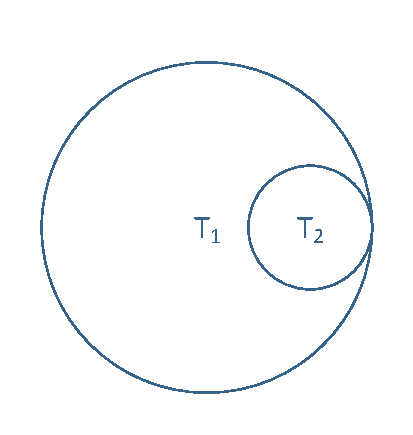
\includegraphics[width=1.31in]{testSuite1.eps}
}
\subfigure[]{
  %  \rule{4cm}{3cm}
    \label{fig:disjoint}
    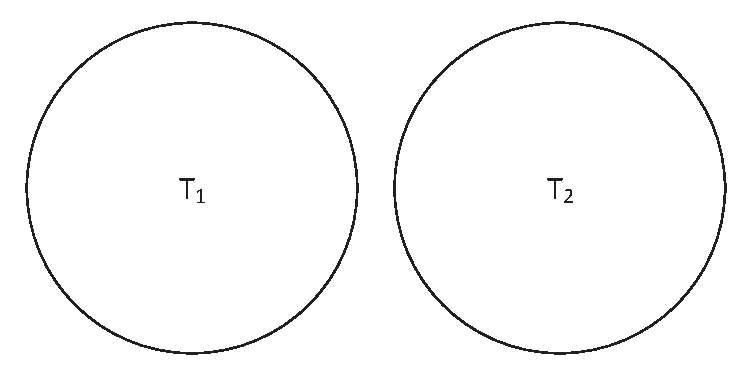
\includegraphics[width=2.01in]{testSuite2.eps}
}
\subfigure[]{
  %  \rule{4cm}{3cm}
    \label{fig:intersect}
    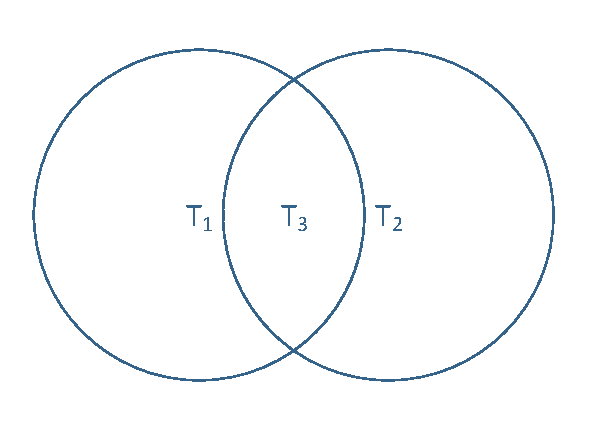
\includegraphics[width=1.81in]{testSuite3.eps}
}
\caption[]{Test Suites relationship}
\label{fig:testSuite}
\end{figure*}

\subsection{Inclusion}

It is the first relationship corresponding to Fig. \ref{fig:inclusion}. We can have the following proposition with two set of test cases which have the inclusion relationship.
%\newtheorem{lemma}{Lemma}
\begin{proposition}
For two set of test cases $T_{l}$ and $T_{k}$, assume that $T_{l} \subset T_{k}$. Then we have
 \begin{displaymath} \forall c_{l} \in \mathcal{C}(T_{l})\,  either\ c_{l} \in \mathcal{C}(T_{k})\ or \exists c_{k} \in \mathcal{C}(T_{k}), s.t., c_{k} \prec c_{l}.
 \end{displaymath}
\end{proposition}

\begin{proof}
Obviously for $\forall c_{l} \in \mathcal{C}(T_{l}) $ we can get $T(c_{l}) \subset T_{l} \subset T_{k}$. According to the proposition 3, we can have $c_{l} \in S(T_{k})$. So this proposition holds as the schema in $S(T_{k})$ either is also in $\mathcal{C}(T_{k})$, or must be the parent of some schemas in $\mathcal{C}(T_{k})$.
\end{proof}

Based on this proposition, in fact, the $c_{k} \in \mathcal{C}(T_{k})$  remains the following three possibilities: 1) $c_{k} \in \mathcal{C}(T_{l})$, or 2) $\exists c_{l} \in \mathcal{C}(T_{l}), s.t.,\ c_{k} \prec c_{l}$, or 3) $\not\exists c_{l} \in \mathcal{C}(T_{l}), s.t., c_{k} \prec c_{l}\ or\ c_{k} = c_{l},\ or\ c_{l} \prec c_{k}$. For the third case, we call $c_{k}$ is \emph{irrelevant} to $\mathcal{C}(T_{l})$

We illustrate these scenarios in Table \ref{example_three_condition}. There are two parts in this table, each part shows two set of test cases: $T_{l}$ and $T_{k}$, which have $T_{l} \subset T_{k}$. For the left part, we can see that the schema in $\mathcal{C}(T_{l})$: (0, 0, -) and (0, -, 0), both are the parent of the schema of the one in $\mathcal{C}(T_{k})$:(0,-,-). While for the right part, the schemas in $\mathcal{C}(T_{l})$: (0, 0, -) and (0, -, 0) are both also in $\mathcal{C}(T_{k})$. Furthermore, one schema in $\mathcal{C}(T_{k})$: (1,1,-) is irrelevant to $\mathcal{C}(T_{l})$.

%in which the left part shows the case that the failure-inducing combinations satisfy the first properties( both (0,0,-) and (0,1,0) subsume (0,-,-)). While the right part give an example to the second properties, as (1,-,-) is irrelevant to any one of (0,0,-) and (0,1,0).

%\begin{proof}
%We proof this by two sides:
%
%for there is one failure-inducing combination is this set, then this condition is similar to proposition 1, and For there is multiple failure-inducing combinations. We can easily find it must exist one failure-inducing combination.
%\end{proof}

\begin{table}
\centering
\tbl{Example of the scenarios\label{example_three_condition}}{
  \begin{tabular}{cc}
$T_{l}$&$T_{k}$ \\ \hline
(0, 0, 0)&(0, 0, 0)\\
(0, 0, 1)&(0, 0, 1) \\
(0, 1, 0)&(0, 1, 0)\\
         &(0, 1, 1) \\ \hline
 $\mathcal{C}(T_{l})$& $\mathcal{C}(T_{k})$ \\ \hline
(0, 0, -)&(0, -, -)\\
(0, -, 0)&		   \\ \hline
  \end{tabular}
  \hspace{1em}
  \begin{tabular}{cc}
$T_{l}$&$T_{k}$\\ \hline
(0, 0, 0) & (0, 0, 0)\\
(0, 0, 1) & (0, 0, 1)\\
(0, 1, 0) & (0, 1, 0)\\
		  & (1, 1, 0)\\
		  & (1, 1, 1)\\ \hline
$\mathcal{C}(T_{l})$& $\mathcal{C}(T_{k})$ \\ \hline
(0, 0, -)&  (0, 0, -)\\
(0, -, 0)&  (0, -, 0)\\
		 &  (1, 1, -)\\  \hline
  \end{tabular}
  }
  \end{table}

%It is noted that as the

\subsection{Disjoint}
This relationship is corresponding to the Fig.\ref{fig:disjoint}, For two different set of test cases, one obvious properties is listed as follows:
\begin{proposition}
 For two set $T_{1}$,$T_{2}$, if $T_{1} \bigcap T_{2} = \emptyset $, we have, $S(T_{1}) \bigcap S(T_{2}) = \emptyset$.
\end{proposition}
\begin{proof}
If $S(T_{1}) \bigcap S(T_{2}) \ne \emptyset$. Without loss of generality, we let $c \in S(T_{1}) \bigcap S(T_{2}) $ we can learn that $T(c)$ must both in $T_{1}$ and $T_{2}$, which is contradiction.
\end{proof}

This properties tells that the minimal schemas of two disjoint test cases should be irrelevant to each other, Table \ref{example_disjoint} list the example of this scenario, we can learn in this table that for two different test cases set $T_{l}$,$T_{k}$, their minimal schemas, i.e., (0, - , 0) and (1, 0, -),(1, -, 0) respectively, are irrelevant to each other.
\begin{table}
\centering
\tbl{Example of disjoint examples \label{example_disjoint}}{
  \begin{tabular}{cc}
$T_{l}$&$T_{k}$ \\ \hline
(0, 0, 0)&  (1, 0, 0)\\
(0, 1, 0)&  (1, 0, 1)\\
		 &  (1, 1, 0)\\  \hline
 $\mathcal{C}(T_{l})$& $\mathcal{C}(T_{k})$ \\ \hline
(0, -, 0)&(1, 0, -)\\
         &(1, -, 0)	\\ \hline
  \end{tabular}
  }
  \end{table}
%Sometimes they can be merged.

\subsection{Intersect}
This relationship is corresponding to the Fig.\ref{fig:intersect}. This scenario is the most common scenario for two set of test cases, but also the most complicated scenario for analysis. For convenience to illustrate the properties of the minimal schemas of this scenario, we assume without of loss of generality that $T_{1} \bigcap T_{2} = T_{3}$ as depicted in Fig.\ref{fig:intersect}. Then we can have the following properties:
%For two different set of test cases, one obvious properties is listed as follows:
%Without loss of generality, For $T_{1}$, their has three possibilities: $for c \in \mathcal{C}(T_{1})$, 1) $c \in  \mathcal{C}(T_{3})$, 2) $c \prec  \mathcal{C}(T_{3})$ 3) $c$ irrelevant to $\mathcal{C}(T_{3})$. This is also for $T_{2}$.

%Let me discuss the combination of them.
\begin{proposition}
 It must have $ \exists c_{1} \in \mathcal{C}(T_{1})\ and\ c_{2} \in \mathcal{C}(T_{2})$. s.t. $c_{1}\ and\ c_{2}$are irrelevant.
\end{proposition}
\begin{proof}
Firstly, we can learn that $\mathcal{C}(T_{1} - T_{3})$ are irrelevant to $\mathcal{C}(T_{2} - T_{3})$, as $(T_{1} - T_{3}) \bigcap (T_{2} - T_{3}) = \emptyset$.

As $\mathcal{C}(T_{1} - T_{3})$ is either identical to some schemas in $\mathcal{C}(T_{1})$ or be parent schemas of them. If some of them are identical, then these identical ones must be irrelevant to $ \mathcal{C}(T_{2})$ as $T_{1} - T_{3} \bigcap T_{2} = \emptyset$. This is also holds if $\mathcal{C}(T_{2} - T_{3})$ is identical to some schemas in $\mathcal{C}(T_{2})$.

Next, if both $\mathcal{C}(T_{1} - T_{3})$  and $\mathcal{C}(T_{2} - T_{3})$ are parent schemas of some of $\mathcal{C}(T_{1})$ and $\mathcal{C}(T_{2})$ respectively, without loss of generality, we make $c_{1-3} \prec c_{1}$, ($c_{1-3}\in\mathcal{C}(T_{1} - T_{3})\ and\ c_{1} \in \mathcal{C}(T_{1})$) and $c_{2-3}\prec c_{2}$, ($c_{2-3}\in\mathcal{C}(T_{2} - T_{3})\ and\ c_{2} \in \mathcal{C}(T_{2})$). Then these corresponding sub-schemas in $\mathcal{C}(T_{1})$ and $\mathcal{C}(T_{2})$, i.e., $c_{1}$ and $c_{2}$ respectively, must also be irrelevant to each other. This is because $T(c_{1}) \supset T(c_{1-3})$ and  $T(c_{2}) \supset T(c_{1-3})$. And as $ T(c_{1-3}) \bigcap  T(c_{2-3}) = \emptyset $  So $T(c_{1})$ and $T(c_{2})$ are neither identical nor subsuming each other.
\end{proof}

For example, Table \ref{example_intersect_irrelevant} shows two test cases interact each other at test case (1,0,0), but their minimal schemas, (1,0,-) and (1,-,0) respectively, are irrelevant to each other.

\begin{table}
\centering
\tbl{Example of Intersect by irrelevant examples \label{example_intersect_irrelevant}}{
  \begin{tabular}{cc}
$T_{1}$&$T_{2}$ \\ \hline
(1, 0, 0) &  (1, 0, 0)\\
(1, 0, 1) &  (1, 1, 0)\\  \hline
 $\mathcal{C}(T_{1})$& $\mathcal{C}(T_{2})$ \\ \hline
(1, 0, -)&(1, -, 0)\\
  \end{tabular}
  }
  \end{table}

\begin{proposition}
If there we can find $\exists c_{1} \in \mathcal{C}(T_{1})\ and\ c_{2} \in \mathcal{C}(T_{2})$, s.t., $c_{1}$ is identical to $c_{2}$, Then it must have $c_{1} = c_{2} \in \mathcal{C}(T_{3})$
\end{proposition}
\begin{proof}
As we get that the identical schema must share the identical test cases, then the only identical test cases between $T_{1}$ and $T_{2}$ is $T_{1} \bigcap T_{2} = T_{3}$. So the only possible identical schemas between $\mathcal{C}(T_{1})$ and $\mathcal{C}(T_{2})$ is in $\mathcal{C}(T_{3})$.
\end{proof}

We must know that this proposition holds when some schemas in $\mathcal{C}(T_{3})$ is identical some schemas in $\mathcal{C}(T_{1})$ and $\mathcal{C}(T_{2})$.

For example, Table \ref{example_intersect_identical} shows two test cases interact each other at test cases (1,1,0)and (1,1,1), and they have identical minimal schemas, i.e., (1,1,-), which is also the minimal schema in $\mathcal{C}(T_{3})$.

\begin{table}
\centering
\tbl{Example of Intersect by identical examples \label{example_intersect_identical}}{
  \begin{tabular}{ccc}
$T_{1}$&$T_{2}$ &$T_{3}$\\ \hline
 (0, 1, 0) & (0, 0, 0) & (1, 1, 0) \\
 (1, 1, 0) & (0, 0, 1) & (1, 1, 1)\\
 (1, 1, 1) & (1, 1, 0) & \\
	       & (1, 1, 1) & \\\hline

 $\mathcal{C}(T_{1})$& $\mathcal{C}(T_{2})$ & $\mathcal{C}(T_{3})$  \\ \hline
(-, 1, 0)&  (0, 0, -) & (1, 1, -)\\
(1, 1, -)&  (1, 1, -) &\\ \hline
  \end{tabular}
  }
  \end{table}

%It must also be that this $c$ must in $T_{3}$, which means that it should not all be children tuples like table.

\begin{proposition}
If there we can find $\exists c_{1} \in \mathcal{C}(T_{1})\ and\ c_{2} \in \mathcal{C}(T_{2})$, s.t., $c_{1}$ is parent-schema of $c_{2}$, Then it must have $c_{1} \in \mathcal{C}(T_{3})$. (and vice versa).
\end{proposition}
\begin{proof}
We have proved previously if two schemas have have subsumes relationship, then their test cases must also have inclusion relationship. And as the only inclusion relationship between  $T_{1}$ and $T_{2}$ is that $T_{1} \subset  T_{3} $  and $T_{2} \subset  T_{3}$. So the parent schemas must be in $\mathcal{C}(T_{3})$.
\end{proof}

It is noted that this proposition holds when holds when some schema in $\mathcal{C}(T_{3})$ is identical in $\mathcal{C}(T_{1})$ (or $\mathcal{C}(T_{2})$), and simultaneously the same schemas in $\mathcal{C}(T_{3})$ must be the parent-schema of the minimal schemas of another set of test cases, i.e., $\mathcal{C}(T_{2})$ (or $\mathcal{C}(T_{1})$).

Table \ref{example_intersect_subsume} illustrates this scenario, in which, the minimal schemas of $T_{1}$: (1,0,-),(1,-,0),which is also the schemas in $\mathcal{C}(T_{3})$, is the parent schema of the minimal schema of $T_{2}$: (1,-,-).

\begin{table}
\centering
\tbl{Example of Intersect by subsume examples \label{example_intersect_subsume}}{
  \begin{tabular}{ccc}
$T_{1}$&$T_{2}$ &$T_{3}$\\ \hline
(0, 1, 0)   & (0, 0, 0) & (1, 0, 0) \\
(1, 0, 0)   & (1, 0, 0) & (1, 0, 1)\\
(1, 0, 1)	& (1, 0, 1) & (1, 1, 0)\\
(1, 1, 0)	& (1, 1, 0) &         \\
        	& (1, 1, 1) & \\ \hline
 $\mathcal{C}(T_{1})$& $\mathcal{C}(T_{2})$ & $\mathcal{C}(T_{3})$  \\ \hline
(-, 1, 0)&  (-, 0, 0) & (1, 0, -)\\
(1, 0, -)&  (1, -, -) & (1, -, 0)   \\
(1, -, 0)&     & \\ \hline
  \end{tabular}
  }
  \end{table}

 It is noted that this three condition can simultaneously appears when two set of test cases interest with each other.%, like Table \ref{example_intersect_all}.

%\begin{table}
%\centering
%\tbl{Example of Intersect by all examples \label{example_intersect_all}}{
%  \begin{tabular}{ccc}
%$T_{1}$&$T_{2}$ &$T_{3}$\\ \hline
%(0, 1, 0)   & (0, 0, 0) & (1, 0, 0) \\
%(1, 0, 0)   & (0, 0, 1) & (1, 0, 1)\\
%(1, 0, 1)	& (1, 0, 0) & (1, 1, 0)\\
%(1, 1, 0)	& (1, 0, 1) &         \\
%        	& (1, 1, 0)\\
%		    & (1, 1, 1)\\ \hline
% $\mathcal{C}(T_{1})$& $\mathcal{C}(T_{2})$ & $\mathcal{C}(T_{3})$  \\ \hline
%(0, 1, 0)&  (0, 0, -) & (1, 0, -)\\
%(1, 0, -)&  (1, -, -) & (1, -, 0)   \\
% (1, -, 0) & & \\ \hline
%  \end{tabular}
%  }
%  \end{table}

%\subsection{Summary of the formal model}
%From the previous analysis, we can learn that for the general intersect test cases-schema model, this is a partial relationship.

\subsection{Identify the MFS}
According to these analysis, we can get that $\mathcal{C}(T_{F_{m}})$ actually is the set of failure-causing schemas of $F_{m}$. Then in theory, if we want to accurately figure out the MFS in SUT, we need to exhaustively execute each possible test case, and collect the failing test cases $T_{F_{m}}$. This is impossible in practice especially when the testing space is too large.

So for traditional FCI approaches, they need to select the subset of the exhaustive test cases, and then either take some assumption to make prediction of the remaining test cases or just give a suspicious rank. As giving a suspicious rank can also be regard as a special case of making prediction(with computing the possibility), so we next only formally describe the mechanism of FCI approaches belong to the first type.
%Formally, we can describe the two ways as following:
We refer the observed failing test case to  $T_{fail_{observed}}$, and refer the remaining test cases the approach predict to be failed as $T_{fail_{predicted}}$. We also denote the actually entire failing test cases as $T_{fail}$. Then the MFS identified by FCI approaches can be depicted as:

MFS = $\mathcal{C}(T_{fail_{observed}} \bigcup T_{fail_{predicted}})$.

%
%\subsubsection{Make assumption}
%Most approaches belong to this partition. Such as one factor one time, FIC\_BS, ELA, Martinez, Nevertheless, we can deduce the following properties:
For each FCI approach, the way it predict the $T_{fail_{predicted}}$ according to observed failing test cases varies, further more, as the test cases it generates is different, the failing test cases observed by different test cases, i.e., $T_{fail_{observed}}$ also varies.  We take an example using OFOT approach to illustrate this formula.

Suppose SUT has 3 parameters, each can take 2 values. And assume the test case (1, 1, 1) failed. Then we can describe the FCI process as Table \ref{ofot-identify}. In this table, test case \emph{t} failed, and OFOT mutated one factor of the \emph{t} one time to generate new test cases: $t_{1}$ -- $t_{3}$, It found the the $t_{1}$ passed, which indicates that this test case break the MFS in the original test case \emph{t}. So the (1,-,-) should be one failure-causing factor, and as other mutating process all failed, which means no other failure-inducing factors were broken, therefore, the MFS in \emph{t} is (1,-,-).

Now let us explain this process with our formal model. Obviously the $T_{fail_{observed}}$ is \{(1,1,1),(1,0,1),(1,1,0)\}. And as having found (0,-,-) broke the MFS, hence by OFOT theory, all the test cases contain (0,-,-) should pass the test cases (This conclusion is built on the assumption that SUT just contain one failure-causing schema).  As a result, {(0,1,1),(0,0,1),(0,1,0),(0,0,0)} should pass the testing. Further, as obviously the test case either passes or fails the testing(we label the skip the testing as a special case of failing), so the remaining test case(1,0,0), will be predicted as failing, i.e., $T_{fail_{predicted}}$ is \{(1,0,0)\}. Taking together, the MFS using OFOT strategy can be described as: $\mathcal{C}(T_{fail_{observed}} \bigcup T_{fail_{predicted}})$ = $\mathcal{C}(\{(1,1,1),(1,0,1),(1,1,0),(1,0,0)\})$ = (1,-,-), which is identical to the one it got previously.

\begin{table}[h]
\tbl{OFOT with our strategy\label{ofot-identify}}{
\begin{tabular}{llllll}
\multicolumn{5}{c}{\bfseries original test case} & \bfseries Outcome \\
 $t$ & \multicolumn{4}{l}{1 \ \ \ \ 1 \ \ \ \  1 } & Fail \\
 \hline
\multicolumn{5}{c}{\bfseries observed} &  \\
$t_{1}$ &\multicolumn{4}{l}{0  \ \ \ \  1 \ \ \ \  1 }& Pass \\
$t_{2}$ &\multicolumn{4}{l}{1  \ \ \ \  0 \ \ \ \  1 } & Fail \\
$t_{3}$ &\multicolumn{4}{l}{1  \ \ \ \  1 \ \ \ \  0 } & Fail \\
\hline
\multicolumn{5}{c}{\bfseries predicted} & \\
$t_{4}$ &\multicolumn{4}{l}{0  \ \ \ \  0 \ \ \ \  1 } & Pass \\
$t_{5}$ &\multicolumn{4}{l}{0  \ \ \ \  1 \ \ \ \  0 } & Pass \\
$t_{6}$ &\multicolumn{4}{l}{1  \ \ \ \  0 \ \ \ \  0 } & Fail \\
$t_{7}$ &\multicolumn{4}{l}{0  \ \ \ \  0 \ \ \ \  0 } & Pass \\
\end{tabular}}
\end{table}
%In this formula, the approach can derive the $T_{fail_{assumed}}$ from the $T_{fail_{observed}}$. For example,  for OFOT, one factor, pass, it can learn all the factor. For colbourn, it can learn from the covering array to be all according the number and t.


\begin{figure}
\centering
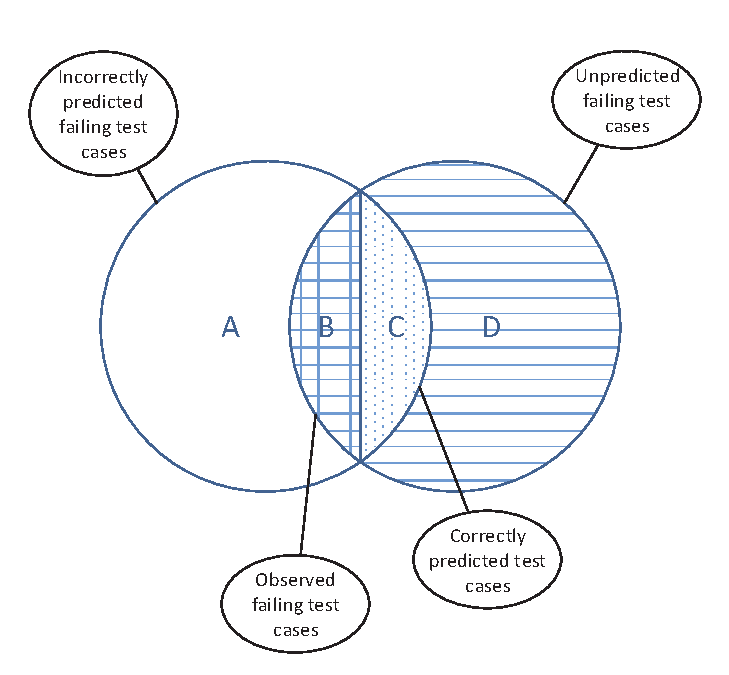
\includegraphics[width=3.31in]{FCI.eps}
\caption{generally modeling of FCI}
\label{fig:fci_process}
\end{figure}

Similarly, other FCI approaches can also be modeled into this formal description. We will not in detail discuss how to model each FCI approach as this is not the point of this paper. It is noted that the test cases FCI predict to be failing is not always identical to the actually failing test cases. In fact, we can generally depict the process of FCI approaches like Fig. \ref{fig:fci_process}.

We can see in this figure, area A denotes the test cases that should be passing ones while it predicted to be failing, area B depicts the test cases that the approach observed to be failing test cases, area C refers to the failing test cases that doesn't to be observed but be predicted to be failing test cases and area D illustrates the failing test cases that neither to be observed nor to be predicted.  This figure is actually one sample of the condition that two set of test cases interest with each other, in specific, area $A \bigcup B \bigcup C $= $T_{1}$, area $D \bigcup B \bigcup C $= $T_{2}$ and area$ B \bigcup C$ = $T_{3}$.

We learned previously this scenario makes the schemas identified in $T_{1}$ biased from the expected MFS in $T_{2}$, in specific, their must be irrelevant schemas between $\mathcal{C}(T_{1})$ and $\mathcal{C}(T_{2})$, which means that FCI approach will identify some minimal schemas that is irrelevant to actual MFS, and must ignore some actual MFS. Moreover, under the appropriate condition list in proposition 3.11 and 3.12, FCI may identify the identical schemas or parent-schema or sub-schema of the actual MFS. So in order to identify the schemas as accurate as possible, the FCI approach needs to make $T_{1}$ as similar as possible to $T_{2}$, specifically, makes area B and area C as large as possible, and make area A as small as possible.

However, even though each FCI approach tries its best to identify the MFS as accurate as possible, masking effects raised from test cases will make their efforts in vain. We next will discusses the masking problem and how it affect the FCI approaches.
%Thus, besides the case that FCI make a perfect prediction, $T_{fail_{observed}} \bigcup T_{fail_{predicted}}$ can either contain $T_{fail}$ or be contained by $T_{fail}$ , or neither of the two circumstances. For the third circumstance, we have the following proposition:
%
%\begin{proposition}
% If neither $T_{m} \subset T_{n}$ nor $T_{n} \subset T_{m}$, then it must be that $c \in $ $\mathcal{C}(T_{n}) $ is irrelevant to $\mathcal{C}(T_{m})$ and must be some $c' \in $ $\mathcal{C}(T_{m}) $ is irrelevant to $\mathcal{C}(T_{n})$  .
%\end{proposition}
%
%\begin{proof}
%We just need to prove the first one, as the latter is equivalent to the first one. The first one can be proven by contradiction.
%
%Assume that for $\forall c \in \mathcal{C}(T_{m})$, have $c either \in \mathcal{C}(T_{n}) $.
%\end{proof}
%
%So either of this three circumstance can make FCI identifying inaccurately as we discussed earlier, and each FCI should avoid these circumstances as much as possible.

%\subsubsection{Proposition of MFS identifying process}

%\subsubsection{Suspicious}
%SP, CTA. The first one will, while the latter not.



\section{Masking effect}
\begin{definition}
A \emph{masking effect} is the effect that while a test case \emph{t} hit a MFS for a particular fault, however, $t$ didn't trigger the expected fault because other fault was triggered ahead which prevents $t$ to be normally checked.

%This masking effect can be presented as $t(F_{b})[F_{a}]$, which means test case \emph{t} should trigger $F_{a}$ if didn't trigger $F_{b}$.
\end{definition}

Taking the masking effects into account, when identifying the MFS for a specific fault, say, $F_{m}$, we should not ignore these test cases which should have triggered $F_{m}$ if they didn't trigger other faults. We call these test cases $T_{mask(F_{m})}$. Hence, the MFS for fault $F_{m}$ should be $\mathcal{C}(T_{F_{m}} \bigcup T_{mask(F_{m})})$

%So in fact, the failure-inducing combination for $F_{m}$ should be the combination which have the test cases $T_{F_{m}} \bigcup T_{mask(F_{m})}$. We call the failure-inducing combinations with considering the masking effects the \emph{perfect failure-inducing combinations}.

As an example, in the motivation example in section 2, the $F_{mask(F_{Ex\ 2})}$  is \{ (7,4,4,5),(11,4,4,5)\}, So the MFS for $Ex 2$ is $\mathcal{C}(T_{F_{Ex\ 2}} \bigcup T_{mask(F_{Ex\ 2})})$, which is (-,-,4,5).
 %taking this test cases into account, we can get the failure-inducing combinations for Ex 1 is .

In practice with masking effects, however, it is not possible to correctly identifying the MFS, unless we fix some bugs in the SUT and re-execute the test cases to figure out $T_{mask(F_{m})}$.

In effect for traditional FCI approaches, without knowledge of  $T_{mask(F_{m})}$,  only two strategies can be adopted when facing the multiple faults problem.
%We will analyse the two strategies under exhaustive testing condition and normal FCI testing condition.

\subsection{Regard as one fault}
The first one is the most common strategy, it doesn't distinguish the faults, i.e., regard all the types of faults as one fault--\emph{failure}, others as the \emph{pass}.

With this strategy, the FCI process turns into identifying the set $\mathcal{C}(\bigcup_{i = 1}^{L}T_{F_{i}})$ , $L$ is the number of all the faults in the SUT. Obviously, $T_{F_{m}} \bigcup T_{mask(F_{m})} \subset \bigcup_{i = 1}^{L}T_{F_{i}}$ . So in this case, by Proposition 3.8, some schemas we get may be the sub-schemas of some of the MFS, or irrelevant to the MFS.

As an example, Suppose we take this strategy in the motivation example, then the MFS we get will be (- 4 4 -) and (- - 4 5). In this example, with \emph{regard as one fault strategy} we consider that schemas (- 4 4 -) and (- - 4 5) should be the cause of both Ex 1 and Ex 2, which in fact, (- 4 4 -) is irrelevant to the MFS of Ex 2 and (- - 4 5) is irrelevant to the MFS of Ex 1.

\subsection{Distinguish faults}
Distinguishing the faults by the exception traces or error code can help make FCI approaches focus on particular fault. Yilmaz in  \cite{yilmaz2013reducing} proposed the \emph{multiple-class} failure characterize method instead of \emph{ternary-class} approach to make the characterizing process more accurately. Besides, other approaches can also be easily extended with this strategy to be applied on SUT with multiple faults.
%We call this strategy \emph{distinguish faults}.

This strategy in fact identifies the set of $\mathcal{C}(T_{F_{m}})$, and as $T_{F_{m}} \bigcup T_{mask(F_{m})} \supset T_{F_{m}} $, consequently, some schemas get through this strategy may be the parent-schema of some MFS. Moreover, some MFS may be irrelevant to the schemas get with this strategy, which means this schemas set ignore these MFS.

It is noted that, the FCI approach listed in motivation example in section 2 actually adopted this strategy, which made the schemas identified for Ex 2: (-,2,4,5), (-,3,4,5) are the parent-schemas of the correct MFS(-,-,4,5).

\subsection{masking effects for FCI approaches}
Previously we just discussed how masking effects affect the exhaustive testing with two strategies. Next we see how traditional FCI process will be interfered with, i.e., how $T_{fail_{observed}}$ and $T_{fail_{predicted}}$ will grow into.
%As the $predicted$ mechanism is not under controlled as it varies in different FCI approaches, what we need to do is ensure the observed is correctly.

The abstract scenario of FCI approaches with masking effects will grow into the Figure \ref{fig:fci_mask}, in which area A, C and D is the same as Figure \ref{fig:fci_process}. Area B is divided into three sub-areas, in which $B_{1}$ is still the observed failing test cases for the current analysed fault, area $B_{2}$ is the test cases triggered other fault which masked the current fault, area $B_{3}$ is the test cases triggered other fault which did not mask the current fault.

\begin{figure}
\centering
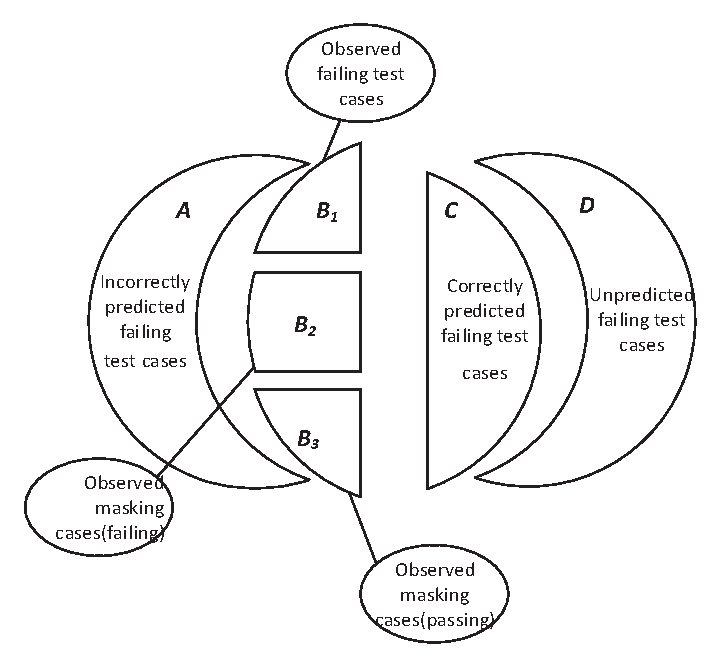
\includegraphics[width=3.31in]{FCI-mask.eps}
\caption{FCI with masking effects}
\label{fig:fci_mask}
\end{figure}

With this model, if we have known which test cases mask the expect fault, i.e., figured out the B2 and B3, then the schemas FCI approach will identify can be described as $\mathcal{C}(A \bigcup B_{1} \bigcup B_{2} \bigcup C)$.  However, as we discussed forehead, this is not possible and what can do is the forehead two strategies.

Then for \emph{regard as one fault} strategy, the MFS traditional FCI identify are $\mathcal{C}(A \bigcup B_{1} \bigcup B_{2} \bigcup B_{3} \bigcup C)$.  And for \emph{distinguish faults} strategy, the MFS is $\mathcal{C}(A \bigcup B_{1} \bigcup C)$.

\subsubsection{using regard as one fault strategy}

For the first strategy: \emph{regard as one fault}, the influence can be described as Figure \ref{fig:fci_mask_regard}. To understand the content of this figure, let us get back to the properties of minimal schemas' relationship between two different set of test cases. We known if we have known masking effects, the result identified by FCI approach, i.e., $\mathcal{C}(A \bigcup B_{1} \bigcup B_{2} \bigcup C)$, grow into the condition of the \emph{intersect} scenario. It means that the minimal schemas get in this condition can be identical, parent-schema, sub-schema, irrelevant to the actual MFS. And then apply the \emph{regard as one fault}, the result is $\mathcal{C}(A \bigcup B_{1} \bigcup B_{2} \bigcup B_{3} \bigcup C)$. It is obviously $A \bigcup B_{1} \bigcup B_{2} \bigcup B_{3} \bigcup C$ $\supset$ $A \bigcup B_{1} \bigcup B_{2} \bigcup C$. So the minimal schema get by this strategy is either the sub-schema or identical to some schemas from the known masking effects, or irrelevant to all the ones. Taking together this two properties together, we will get Figure \ref{fig:fci_mask_regard}.

\begin{figure}
\centering
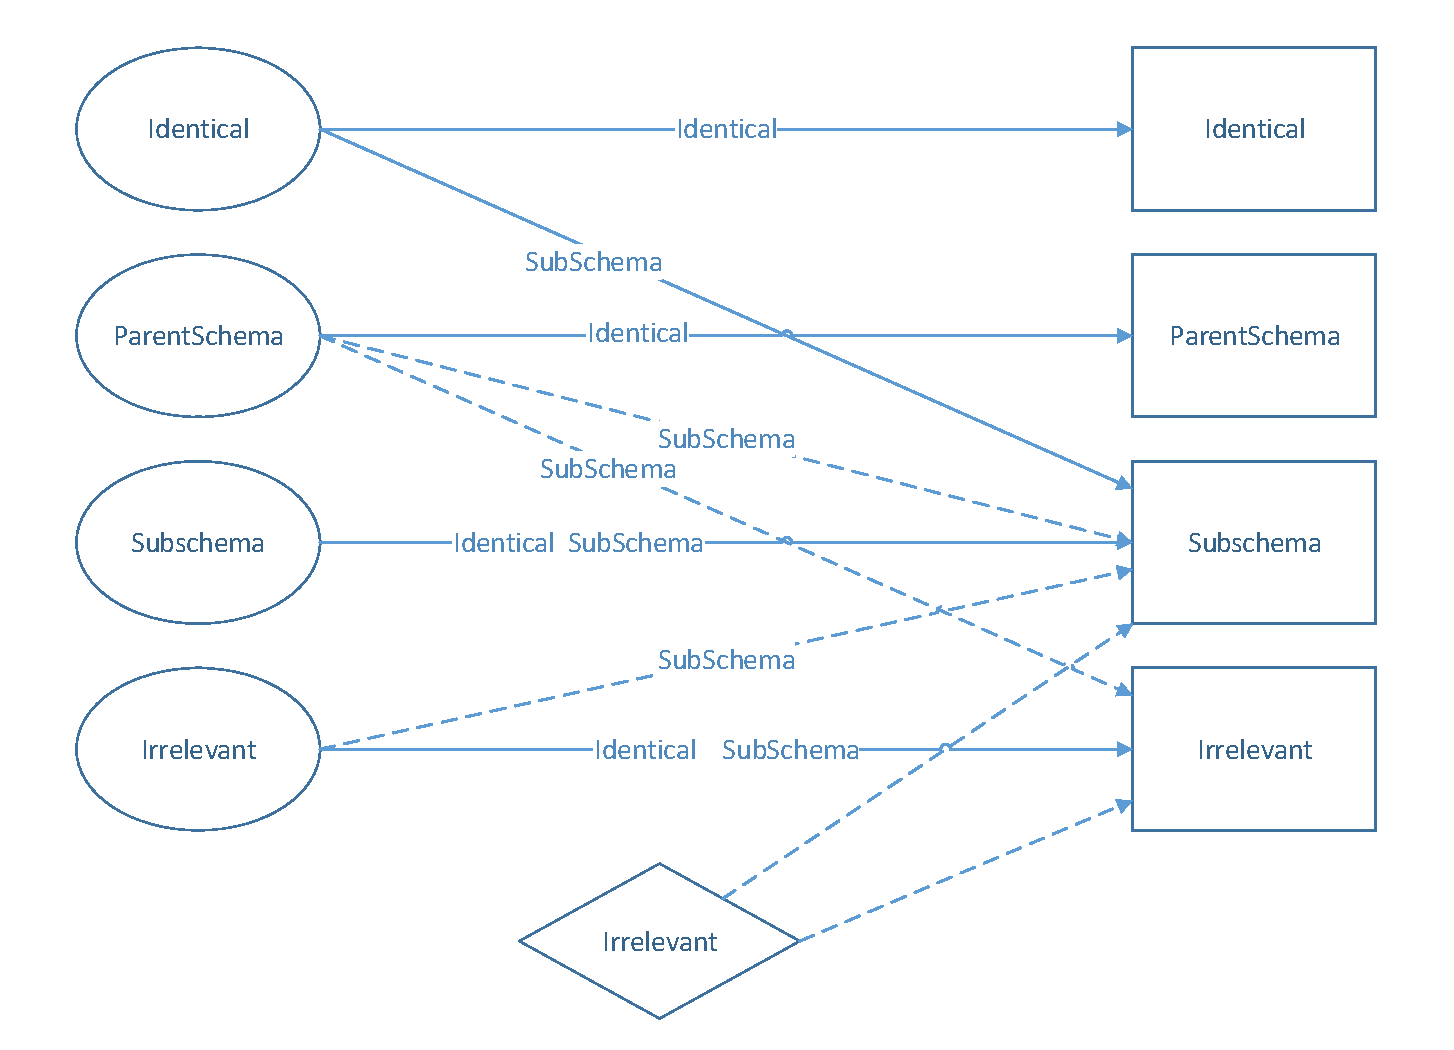
\includegraphics[width=4.31in]{fci-mask-influence2.eps}
\caption{masking effects influence on FCI with regard as one fault}
\label{fig:fci_mask_regard}
\end{figure}

Now we can easily understand this figure, the left column in this figure means the schemas identified by FCI knowing masking effects at ahead, then as we take the \emph{regard as one fault} strategy, the schemas will be either sub-schema or identical or irrelevant to the previous schemas. So if we originally get the identical schema to actual MFS with knowing masking effects, then after applying the strategy, if we still get the identical as originally identified, then the final result is still identical to the actual MFS, else if we get the sub-schema to the originally identified, then the final result is the sub-schema to the actual MFS. In this figure, the directed-line represent the changing method from the original identified, and the right column represent the final transformed result against the actual MFS.

Some transformation in this figure is obviously, such as original sub-schema changing by sub-schema is still the sub-schema. Next we just prove the transformation that is hard to understand.

\begin{proposition}
Original parent-schema, the sub-schema must be irrelevant.

\end{proposition}

%As for the first one, there are three possibilities, and then less one area make it father schema or identical to the original ones. Then the influence will dive into figure \ref{fig:fci_mask_regard}. The first two is easy to understand, that identical with identical is also identical, father .
%The hard to understand is the sub and father, and irrelevant father.

\begin{proof}
Without loss of generality, we assume $c$ is the parent schema to the actual MFS. Based on previous proposition 3.12, we have $c \in \mathcal{C}(T_{3})$, which means $c \in \mathcal{C}(B_{1} \bigcup B_{2})$.

Then apply \emph{regard as one fault}, i.e., the $B_{3}$ is appended for analysis. Now if we find some schema, say $c' \prec c$,s.t., $c' \in \mathcal{C}(A \bigcup B_{1} \bigcup B_{2} \bigcup B_{3})$, then $T(c')$ must contain some test cases in in $B_{3}$ (if not, $c$ must be the minimal schemas).

This time, for $c'$, as $T(c')$ contain other test cases besides $T_{failing}$, then $c'$ is not the parent-schema or identical of any MFS. And $c'$ is also not possible the sub-schema of some MFS. This is because, based on proposition 3.12, if exist $c_{m}$ is the parent-schema of some identified minimal schema,then the MFS must have $c_{m} \in \mathcal{C}(T_{3})$, and $T(c_{m}) \subset T(c')$. As we see all the set $T(c')$ contained in the failing test cases is $T(c)$. So either $T(c) \supset T(c_{m})$ or  $T(c) = T(c_{m})$, which means that $c \prec c_{m}$ or  $c = c_{m}$, this is impossible as $c$ is the parent-schema of some MFS, and $c_{m}$ is the MFS. So $c'$ is not possible the sub-schema of some MFS.

Thus, at last $c'$ must be irrelevant to the actual MFS.
\end{proof}

\begin{proposition}
Original irrelevant, the sub-schema must be irrelevant.

\end{proposition}

\begin{proof}
Without loss of generality, we assume $c$ is irrelevant to the actual MFS. Then $T(c)$ must contain some other test cases in $A$. After using the  \emph{regard as one fault} strategy, the same as the previous proposition, if we have $c' \prec c$, then $T(c')$ must append some test cases in $B_{3}$.

Still $c'$ is not possible the parent-schema or identical ones. If we assume there is MFS $c_{m}$ s.t., $c' \prec c_{m}$, we must have $T(c') \supset T(c_{m})$. Then as $T_{c'}$ is just some test case in $B_{3}$ with $T_{c}$, so we must also have$T_{c} \supset T(c_{m})$, which means $c \prec c_{m}$, which is not possible, as $c$ is irrelevant to the MFS.

Thus,$c'$ must be irrelevant.
\end{proof}

For the newly derived irrelevant ones, we can have

\begin{proposition}
Newly irrelevant ones must be irrelevant or subsume to MFS.

\end{proposition}

\begin{proof}
Without loss of generality, we get new $c$ irrelevant to $\mathcal{C}(A \bigcup B_{1} \bigcup B_{3})$. Similarly as previous propositions, it must have that $T(c)$ contain some test cases in $B_{3}$.

So as T(c) contain other test cases, then $c$ neither be the parent-schema nor be the identical ones. %Then we assume some MFS $c_{m}$, s.t., $c \prec c_{m}$, s.t., $T(c) \supset T(c_{m})$, So the $T(c_{m})$ must be included in $T_{3}$. So previously we will have,

\end{proof}


\subsubsection{using distinguish strategy}

%Another point need to be noted is that this also mean some ignored ones(As MFS irrelevant to the set). That with this strategy, will get more ignored ones.

And for the second strategy: \emph{distinguish faults}, the influence can be described as Figure \ref{fig:fci_mask_distinguish}.
\begin{figure}
\centering
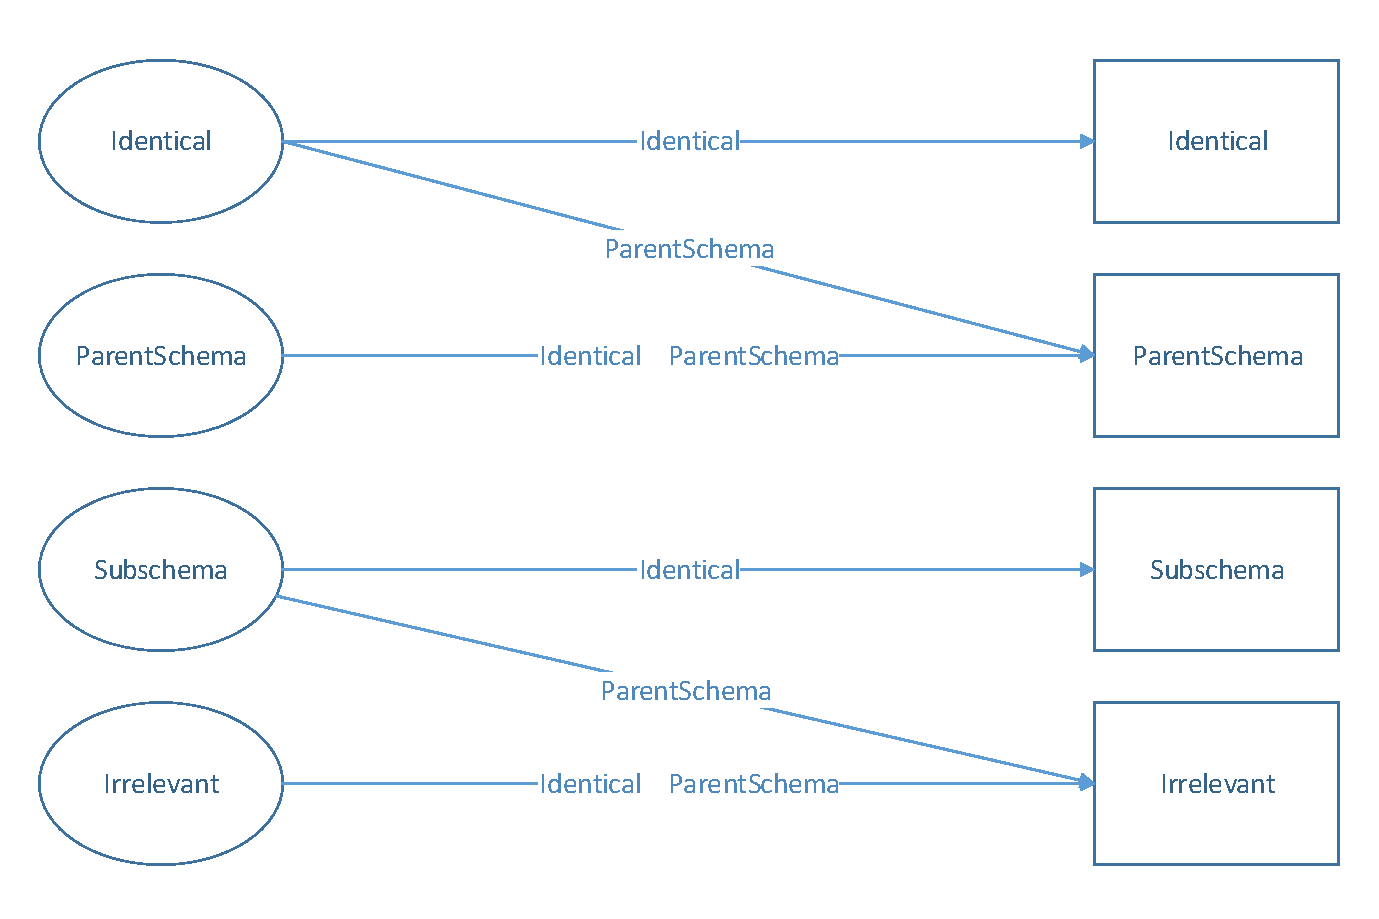
\includegraphics[width=4.31in]{fci-mask-influence.eps}
\caption{masking effects influence on FCI with distinguish faults}
\label{fig:fci_mask_distinguish}
\end{figure}

This figure is organised the same way as figure \ref{fig:fci_mask_regard}. As with distinguish strategy, the minimal schemas identified are actually $\mathcal{C}(A \bigcup B_{1} \bigcup C)$.  Obviously $A \bigcup B_{1} \bigcup C \subset A \bigcup B_{1} \bigcup B_{2} \bigcup C $. So this transformation should be either parent-schema or identical to the originally schemas.

Similarly, we just give the proof of some transformation that is not so obviously.
\begin{proposition}
Original sub-schema, the parent-schema must be irrelevant.

\end{proposition}
\begin{proof}
Without loss of generality, we assume $c$ is sub-schema to the actual MFS, say, $c_{n}$. Then $T(c)$ must contain some other test cases in $A$. After using the  \emph{distinguish  faults} strategy, if we have $c \prec c'$, then $T(c')$ must lose some test cases in $B_{2}$.(If not so, there must be no c').

So as it contain other test cases in $A$ and lose some test case in $B_{2}$. It cannot be the parent and identical to the MFS. If it is sub-schema of some MFS, say $c_{m}$. Then we must have $T(c_{m}) \subset T(c_{n})$. As Both $c_{m}$ and $c_{n}$ are MFS, which contradicts.
\end{proof}


\begin{proposition}
Original identical-schema, the parent-schema must be irrelevant.

\end{proposition}
\begin{proof}
Without loss of generality, we assume $c$ is irrelevant to the actual MFS, say, $c_{n}$. Then $T(c)$ must contain some other test cases in $A$. After using the  \emph{distinguish  faults} strategy, if we have $c \prec c'$, then $T(c')$ must lose some test cases in $B_{2}$.(If not so, there must be no c').

So as it contain other test cases in $A$ and lose some test case in $B_{2}$. It cannot be the parent and identical to the MFS. If it is sub-schema of some MFS, say $c_{m}$. Then we must have $T(c_{m}) \subset T(c_{n})$. As Both $c_{m}$ and $c_{n}$ are MFS, which contradicts.
\end{proof}

Another point need to be noted is that this transformation also mean some ignored ones(As MFS irrelevant to the set).
%So what this two mutation than is , we first learn that
%
%So actually, when encountering masking effects, both this two strategies is not good.


%Previous analysis just based on the the observed changed, in fact, the if we changing the analysis, the pridicted and observed will aslo be changed?

%In fact, the masking effects firstly change the $T_{fail_{observed}}$, as masking effects, FCI either will identify $T_{fail_{observed}}$ less or more than it expected to be, as a consequence, regardless of $T_{fail_{predicted}}$ can be, masking effects makes FCI approaches never reach a perfect result, i.e., accurately and completely find each MFS.
%
%Secondly, as $T_{fail_{observed}}$ changed, $T_{fail_{predicted}}$ consequently changed. As a result, if $T_{fail_{predicted}}$ it can accurate predict without masking effects, then masking effects obviously makes the FCI approaches worse. However, if it originally cannot predicted inaccurately, then this changing will have a possibility make the $T_{fail_{observed}}$ changing better, and of course, it also can have a possibility make the $ T_{fail_{predicted}}$ changing worse.

\subsection{Summary of the masking effects on FCI approach}
From the analysis of formal model, we can learn that masking effects do influence the FCI approaches, worse more, both strategies \emph{regard as one fault} and \emph{distinguish faults} are harmful, which specifically the former comparing the knowing masking effects have a large possibility that get more sub-schemas of the actual MFS and get more schemas which are irrelevant to the MFS, while the latter may get more parent schemas of the MFS and get more irrelevant MFS and also may ignore some of them.

Note that our discussion is based on that SUT is a deterministic software, i.e., the random failing information of test case will be ignored. The non-deterministic problem will complex our test scenario, which will not be discussed in this paper.

\section{Test case replacing strategy}
%Previous section formally studied the case that under the masking effects, neither regarding as one fault approach nor distinguishing faults approach is not accurate .
The main reason why both strategies cannot accurately identify the MFS is that we cannot figure out the $T(mask_{F_{m}})$.  As $T(mask_{F_{m}}) \subset \bigcup_{i = 1 \& j \neq m }^{L}T_{F_{i}}$, in order to weaken the influence of $T(mask_{F_{m}})$, we need to reduce the number of test cases that trigger other faults as much as possible.

In the exhaustive testing, as all the test cases will be used to identify the MFS, there is no room left to improve accuracy. However, when just needing to select part of the whole test cases to identify MFS, which is practical and sometimes the only solution for large-scale SUT, we can adjust the test cases we need to use by selecting proper ones so that we can limit the size of $T(mask_{F_{m}})$ to be as small as possible.

\subsection{Replace test case triggering unexpected fault}

The basic idea is to pick the test cases that trigger other faults and generate newly test cases to replace them. These regenerated test cases should either pass in the execution or trigger $F_{m}$. The replacement must satisfy that the newly generated ones will not negatively influence the original identifying process.

Commonly, when we replace the test case that triggers unexpected fault with a new test case, we should keep some part in the original test case, we call this part as \emph{fixed part}, and mutate other part with different values from the original one. For example, if a test case (1,1,1,1) triggered an unexpected fault, and the fixed part is (-,-,1,1), then we can replace it with a test case (0,0,1,1) which may either pass or trigger expected fault.

The \emph{fixed part} can be the factors that should not be changed in the OFOT algorithm, or the part that should not be mutated of the test case in the last iteration for FIC\_BS algorithm.

It is noted that this replacement may need to execute multiple times for one fixed part as we could not always find a test case that happen to satisfy our requirement. Our previous work just randomly choose test cases until find one satisfied test case. That brute method may be simple and really works, but also may need too many test cases to get one satisfied test case, which contain many wasteful trial. So to handle this problem and reduce the cost, we augment our approach with one data structure -- "suspicious set", which during the originally test, record the test cases that trigger other test cases and next replacement process will consult this set to avoid some test cases with a high probability to trigger other faults.

The process of replacing a test case with a new one keeping some fixed part is depicted in Algorithm 1:

\begin{algorithm}[t]
\SetAlgoNoLine
\KwIn{ the original test case $t_{original}$,fault type $F_{m}$,fixed part $s_{fixed}$, values set that each option can take $Param$}
\KwOut{ $t_{new}$ the regenerate test case,The frequency number }
$index$ = 0; $FreNum_{\alpha}$ = -1\;
\While{\textbf{not} MeetEndCriteria()}{
       $s_{mutant} \leftarrow t_{original} - s_{fixed}$\;
       \ForAll {$opt \in s_{mutant}$}{
          $i = getIndex(Param,opt) $\;
           $opt \leftarrow opt' \ s.t.\ opt' \in Param[i]\ and\ opt' != opt$\;
          }
       $t_{new} \leftarrow s_{fixed} \bigcup s_{mutant} $\;
       $result \leftarrow execute(t_{new})$\;
        \eIf {$result == PASS\ or\ result ==  F_{m}$}{
         \Return $t_{new}$\;
           }{
         continue\;
         }
       }
       \Return \emph{null}

\caption{replace test cases triggering unexpected faults}
\label{alg:one}
\end{algorithm}


The inputs for this algorithm consists of a test case which trigger an unexpected fault -- $t_{original}$, the fixed part which we want to keep from the original test case -- $s_{fixed}$ , the fault type which we currently focus on -- $F_{m}$, and the values sets that each option can take from respectively.  The output of this algorithm is a test case $t_{new}$ which either trigger the expected $F_{m}$ or passes.

This algorithm is a loop(line 1 - 14) containing two parts:

The first part(line 2 - 7) generates a new test case which is different from the original one. This test case will keep the fixed part (line 7), and just mutate the factors which are not in that part(line 2). The mutation for each factor works by selecting one legal value(by random) which is different from the original one(line 3 - 6). The generated newly test case must be different from each iteration(we implemented it by hashing method).

Second part is to check whether the newly generated test case is as expected(line 8 - 13). We first execute the SUT under the newly generated test case(line 8) and then check the executed result. Either the test case passes or triggers the same fault -- $F_{m}$ meets the requirement(line 9), and if so we will directly return this test case(line 10). Otherwise, we will repeat the process, i.e., generate newly test case and check again(line 11 -12).

It is noted that the loop has another exit besides we find an expected test case(line 10), which is when the function \emph{MeetEndCriteria()} returns \emph{true}(line 1). We didn't explicitly show what the function \emph{MeetEndCriteria()} is like, because this is depending on the computing resource and how accurate you want to the identifying result to be. In detail, if you want to get a high quality result and you have enough computing resource, you can try much times to get the expected test case, otherwise, a relatively small number of attempts is recommended.

In this paper, we just set 3 as the biggest repeated times for this function. When it ended with \emph{MeetEndCriteria()} is true, we will return null(line 15), which means we cannot find an expected test case.

\subsection{A case study with the replacing strategy}
%Next we will take the FCI approach--OFOT algorithm as the subject to see how our approach works on them.

Suppose we have to test a system with four parameters, each has three options. And when we execute the test case (0 0 0 0), a failure--$Err 1$ is triggered. Next we will use the FCI approach -- OFOT with replacing strategy to identify the MFS for the $Err 1$. The process is listed in Table \ref{ofot-aug}. In this table, the test case which are labeled with a deleted line represent the original test case generated by OFOT, and it will be replaced by the regenerated test case which are labeled with a wave line under it.

From table \ref{ofot-aug}, we can find the algorithm mutates one factor to take the different value from the original test case one time. Originally if the test case encounter the result different from the expected error, OFOT will derive the fact that the MFS was broken, in another word, if we change one factor and it does not trigger the expect error, we will label it as one failure-inducing factor, after we changed all the elements, we will get the MFS. For this case, if we take the \emph{regard as one fault} strategy, then the MFS we got is (- - - 0) because the last case passed test case while the remaining test cases triggered either $Err 1$ or $Err 2$(regard as one fault).  Additionally when we take the \emph{distinguish faults} strategy, the MFS obtained is (- 0 0 0) as when we changed the second factor, third factor and the fourth factor, it didn't trigger the $Err 1$ ( for second factor, it triggered $Err 2$ and for the third and fourth, it passed).

% So if we do not regenerate the test configuration (0 2 0 0), we will get the MFS -- ( - 0 0 0) for the err 1(which are also labeled with a delete line).

However, if we replace the test case $t_{2}$--(0 1 0 0) with $t_{2}'$--(0 2 0 0) which triggered err 1 (in this case, the fixed part of the test case is (0, - - -)), and replace the test case $t_{3}$--(0 0 1 0) with $t_{3}'$--(0 0 2 0) which passed, we will find that only when we change the third and fourth factor will we broke the MFS for err 1, therefore,  the failure-inducing combination for err 1 should be (- - 0 0).


\begin{table}[h]
\tbl{OFOT with our strategy\label{ofot-aug}}{
\begin{tabular}{llllll}
\multicolumn{5}{c}{\bfseries original test case} & \bfseries fault info \\
 $t$ & \multicolumn{4}{l}{0 \ \ \ \ 0 \ \ \ \  0 \ \ \ \  0 } & Err 1 \\
 \hline
$t_{1}$ &\multicolumn{4}{l}{1  \ \ \ \  0 \ \ \ \  0  \ \ \ \  0 }& Err 1 \\
$t_{2}$ &\multicolumn{4}{l}{\sout{0  \ \ \ \  1 \ \ \ \  0  \ \ \ \  0 }} & \sout{Err 2} \\
$t_{2}'$ &\multicolumn{4}{l}{\uwave{0  \ \ \ \  2 \ \ \ \  0  \ \ \ \  0}} & \uwave{Err 1} \\
$t_{3}$ &\multicolumn{4}{l}{\sout{0  \ \ \ \  0 \ \ \ \  1  \ \ \ \  0 }} & \sout{Err 2} \\
$t_{3}'$ &\multicolumn{4}{l}{\uwave{0  \ \ \ \  0 \ \ \ \  2  \ \ \ \  0}} & \uwave{Pass} \\
$t_{4}$ &\multicolumn{4}{l}{0  \ \ \ \  0 \ \ \ \  0  \ \ \ \  1} & Pass \\
\hline
\multicolumn{3}{l}{\bfseries regard as one fault} &  \multicolumn{3}{l}{\bfseries replacing strategy} \\
\multicolumn{3}{l}{ ( -  \ \ \  - \ \ \  -  \ \ \ 0) } &\multicolumn{3}{l}{ ( -  \ \ \  - \ \ \  0  \ \ \ 0) } \\
\multicolumn{3}{l}{\bfseries distinguish faults} &\multicolumn{3}{l}{} \\
\multicolumn{3}{l}{(  -  \ \ \  0 \ \ \  0  \ \ \ 0 )} &\multicolumn{3}{l}{} \\
\end{tabular}}
\end{table}


\subsection{Complexity analysis}
This complexity lay on two facts: the number of test cases triggered other faults which need to be replaced, and the number of test cases that need to be selected to generate a non-masking-effects test case to replace a test case that trigger the other fault. The last complexity is the product of this two factor.

The first factor is according to the extra test cases that needed to identify the MFS in the failing test cases, this number varies in different FCI approaches, Table \ref{extra-testcases-complexisty} list the number of test cases that each algorithms that needed to get the MFS. In this table, \emph{d} indicates the number of MFS in the SUT. \emph{k} means the number of the parameters of the SUT. \emph{t} is the degree of the MFS in the SUT. \emph{c} is an upper bond, satisfies, $d \leq \frac{c}{2} loglog k$. \emph{v} is the number of values one parameter can take.

\begin{table}
\centering
\tbl{The number of test cases each FCI approach needed to identify MFS\label{extra-testcases-complexisty}}{
  \begin{tabular}{c | c}
\bfseries Method & \bfseries number of test cases to identify MFS\\ \hline
Charles ELA &  \\
Martinez with safe value \cite{martinez2008algorithms,martinez2009locating} & $O(\hat{d}log k + \hat{d}^{2})$ \\
Martinez without safe values \cite{martinez2008algorithms,martinez2009locating} & $O(d^{2} + dlog k + log^{c} k)$  \\
Martinez' ELA \cite{martinez2008algorithms,martinez2009locating} &  $ds^{v}log k$\\
Shi SOFOT \cite{shi2005software}& $k$ \\
Nie OFOT \cite{nie2011minimal} & $kd$\\
Ylimaz classification tree & \\
FIC \cite{zhang2011characterizing} &  $k$ \\
FIC\_BS \cite{zhang2011characterizing}& $t(log k + 1) + 1$\\
Ghandehari's suspicous based  \cite{ghandehari2012identifying}& \\
TRT \cite{niu2013identifying}&  \\
  \end{tabular}
  }
  \end{table}

It must be noted that each algorithm may be limited to some restrictions to identify the result, details can be saw in \cite{zhang2011characterizing}.

To get the complexity of the second factor, we need to figure out the possibility that a test case that could trigger other fault. The first thing we need to care is the \emph{fixed} part, as the additional generated test case should somehow contain this part. This complexity also varies in the adaptive method and non-adaptive. Adaptive method, is commonly identify the MFS in a existed failing test case, while non-adaptive will not limited to this existed failing test case. We can generate $v^{k - p}$  (\emph{p} is the number of factors in the \emph{fixed} part)possible test cases that contain the \emph{fixed} part. Apart from the one that need to be replaced, there remain $v^{k - p} - 1$. For non-adaptive method, in theory, all the remained $v^{k - p} -1$ can trigger other faults, which indicates the complexity is $O(v^{k - p} - 1)$. While for adaptive approach, as the $\emph{fixed}$ part is derived from the existed failing test case, which in fact make the test cases to be selected one more less (the existed one), so the complexity is  $O(v^{k - p} - 2)$.

It is noted that exponential factor $k - p$ directly affects the complexity of the second factor, the more $p$ is, the less test cases could be generated. For different approach, $p$ is different. As for OFOT, $p$ is a fixed number, which is $k - 1$, it is the minimal number of the test cases we need to give. While for FIC\_BS, the $p$ varies in the test cases it generates, ranges from $k-1$ to $1$. While for non-adaptive, as the $fixed $ part is the coverage, we list them as $t$ and this is also for suspicious. We list them all in Table \ref{fixed-part-complexisty}.

\begin{table}
\centering
\tbl{The complexity of second part\label{fixed-part-complexisty}}{
  \begin{tabular}{c | c}
\bfseries Method & \bfseries fixed part\\ \hline
Charles ELA &   $O(v^{k - t} - 1)$\\
Martinez with safe value \cite{martinez2008algorithms,martinez2009locating} &$O(v - 2) ~ O(v^{k - 1} - 2)$\\
Martinez without safe values \cite{martinez2008algorithms,martinez2009locating} &$O(v - 2) ~ O(v^{k - 1} - 2)$  \\
Martinez' ELA \cite{martinez2008algorithms,martinez2009locating} & $O(v^{k - t} - 1)$\\
Shi SOFOT \cite{shi2005software}& $O(v - 2) $\\
Nie OFOT \cite{nie2011minimal} & $O(v - 2)$\\
Ylimaz classification tree & $O(v^{k - t} - 1)$\\
FIC \cite{zhang2011characterizing} &  $O(v - 2) ~ O(v^{k - 1} - 2)$\\
FIC\_BS \cite{zhang2011characterizing}& $O(v - 2) ~ O(v^{k - 1} - 2)$\\
Ghandehari's suspicous based  \cite{ghandehari2012identifying}&$ O(v^{k - t} - 2)$\\
TRT \cite{niu2013identifying}&$ O(v - 2) ~ O(v^{k - 1} - 2) $\\
  \end{tabular}
  }
  \end{table}

The production of this two complexity is the final complexity for our approach. This result is a upper bond, most times the system will just contain small size of faults which will significantly not reach this bond. Also, if a system with too many bugs that make the replacement too costly will just need to rewrite instead of identifying. Further more our "suspicious set" will largely reduce the replacement cost comparing with previous work, which will be validated in the empirical study later.
%
%This complexity is well lay on the number of faults and the magnitude and location of the MFS of each schema, we only analysis the average performance of our approach. Also this approach also lay on the number of tests need to be executed about each algorithm.


\section{empirical studies}
We conducted several empirical studies to address the following questions:

\textbf{Q1}: Do masking effects exist in real software when it contain multiple faults?

\textbf{Q2}: How much do traditional approaches suffer from these real masking effects?

\textbf{Q3}: Can our approach do better than traditional approaches when facing these masking effects?

\textbf{Q4}: Comparing with previous work, do our new approach get improvement in handling effects and limiting the costs(reducing extra test cases).

\textbf{Q5}: Does voting system that consists of different approaches can make improvements?
%
%Specifically, section 6.1 surveyed several open-source software to gain a insight of the existence of multiple faults and their masking effects. Section 6.2 directly applied three MFS-identifying programs on the surveyed software and analysis their results. Section 6.3 applied our approach on the software and a comparison with traditional approaches will be discussed. Section 6.4 discuss the threats to validity of our empirical studies.

\subsection{The existence of masking effects}
In the first study, we surveyed two open-source software to gain an insight on the existence of multiple faults and their effects. The software under study are: HSQLDB and JFlex, the first is a database management software written in pure java and the second is a lexical analyser generator. Each of them contain different versions. All the two subjects are highly configurable so that the options and their combination can influence their behaviour. Additionally, they all have developers' community so that we can easily get the real bugs reported in the bug tracker forum. Table \ref{software description} lists the program, the number of versions we surveyed, number of lines of uncommented code, number of classes in the project and the bug's id of each software we studied.

\begin{table}\renewcommand{\arraystretch}{1.3}
\tbl{Software under survey\label{software description}}{
\begin{tabular}{c|c|c|c|c} \hline
software & versions & LOC & classes & bug pairs\footnote{ http://sourceforge.net/p/hsqldb/bugs
http://sourceforge.net/p/jflex/bugs  } \\ \hline

HSQLDB  &2.0rc8 & 139425 & 495 &  \#981 \& \#1005\\
	   &2.2.5 & 156066 & 508 & \#1173 \&  \#1179\\
	    &2.2.9 & 162784 &525 & \#1286 \& \#1280\\
JFlex  &1.4.1 &  10040 &58 & \#87 \& \#80 \\
      &1.4.2 &  10745 &61 &  \#98 \& \#93  \\
\hline\end{tabular}
}
\end{table}
%http://hsqldb2.0.sourcearchive.com/downloads/2.0.0$\scriptsize{\sim}$rc8/

%\footnote{http://sourceforge.net/projects/jflex/files/jflex}

% \footnote{http://sourceforge.net/projects/hsqldb/files/hsqldb/ }

\subsubsection{Study setup}
We first looked through the bug tracker forum of each software and picked some bugs which are caused by the options combination. For each bug, we will derive its failure-inducing combinations by analysing the bug description report and its attached test file which can reproduce the bug. For example, through analysing the source code of the test file of bug\#981 for HSQLDB, we found the failure-inducing combinations for this bug is: (\emph{preparestatement}, \emph{placeHolder}, \emph{Long string}), this three factors together form the condition on which the bug will be triggered. These analysed results will be regarded as the ``prior failure-inducing combinations" later.

We further selected pairs of bugs belong to the same version and merged their test file, so that we can reproduce different faults through controlling the inputs to that merged test file. This merging manipulation varies with the pair of bugs we selected, and for each pair of bugs, the source code of the merging file as well as other detailed experiment information is available at-- https://code.google.com/p/merging-bug-file.

Next we built the input model which consist of the options related to the failure-inducing combinations and additional noise options. The detailed model information is in Table \ref{modelHSQLDB} and \ref{modelJFlex} for HSQLDB and JFLex respectively. Each table is organised into four groups: 1)``common options", which lists the options as well as their values under which every version of this software can be tested. 2)``common boolean options", which lists additional common options whose values type is boolean. 3)``specific options", under which only the specific version of that software can be tested. 4)``configure space", which depicts the input model for each version of the software.

We then generated the exhaustive test suite consist of all the possible combinations of these options and under each of them we executed the merged test file. We recorded the output of each test case to observe whether there are test cases contain prior failure-inducing combination but do not produce the corresponding bug.



\begin{table}[h]
\tbl{Input model of HSQLDB\label{modelHSQLDB}}{
\begin{tabular}{llllll}
\multicolumn{3}{c}{\bfseries common options} & \multicolumn{3}{c}{\bfseries values}  \\
  \hline
 \multicolumn{3}{c}{Server Type} & \multicolumn{3}{c}{server, webserver, inprocess}  \\
  \multicolumn{3}{c}{  existed form}  & \multicolumn{3}{c}{mem, file}  \\
   \multicolumn{3}{c}{ resultSetTypes}  & \multicolumn{3}{c}{forwad, insensitive, sensitive} \\
   \multicolumn{3}{c}{ resultSetConcurrencys}  & \multicolumn{3}{c}{read\_only, updatable}  \\
  \multicolumn{3}{c}{  resultSetHoldabilitys}  &\multicolumn{3}{c}{ hold, close} \\
  \multicolumn{3}{c}{ StatementType }  &\multicolumn{3}{c}{statement, prepared}  \\
    \hline
   \multicolumn{6}{c}{  \bfseries common boolean options }\\
    \hline
    \multicolumn{6}{c}{   sql.enforce\_strict\_size, sql.enforce\_names, sql.enforce\_refs}\\
      \hline
   \bfseries versions &   \multicolumn{2}{c}{  \bfseries specific options}  & \multicolumn{3}{c}{  \bfseries values}\\
    2.0rc8 & \multicolumn{2}{c}{ more} & \multicolumn{3}{c}{ true, false}\\
      & \multicolumn{2}{c}{ placeHolder} & \multicolumn{3}{c}{ true, false }\\
      & \multicolumn{2}{c}{ cursorAction }& \multicolumn{3}{c}{ next,previous,first,last}\\
    2.2.5 &\multicolumn{2}{c}{  multiple} & \multicolumn{3}{c}{ one, multi, default}\\
       & \multicolumn{2}{c}{ placeHolder} & \multicolumn{3}{c}{ true, false}\\
    2.2.9 & \multicolumn{2}{c}{ duplicate }& \multicolumn{3}{c}{ dup, single, default}\\
     & \multicolumn{2}{c}{ default\_commit} & \multicolumn{3}{c}{ true, false} \\
        \hline
   \bfseries versions &  \multicolumn{3}{c}{\bfseries Config space}&\multicolumn{2}{c}{}\\
   \hline
   2.0rc8 & \multicolumn{3}{c}{$2^{9} \times 3^{2} \times 4^{1}$} &\multicolumn{2}{c}{} \\
    2.2.5 &  \multicolumn{3}{c}{$2^{8} \times 3^{3}$ } & \multicolumn{2}{c}{} \\
     2.2.9 & \multicolumn{3}{c}{$2^{8} \times 3^{3}$} &\multicolumn{2}{c}{}
\end{tabular}
}
\end{table}

\begin{table}[h]
\tbl{Input model of JFlex\label{modelJFlex}}{
\begin{tabular}{llllll}
\multicolumn{3}{c}{\bfseries common options} & \multicolumn{3}{c}{\bfseries values}  \\
  \hline

 \multicolumn{3}{c}{ generation} & \multicolumn{3}{c}{switch, table, pack}  \\
  \multicolumn{3}{c}{  charset}  & \multicolumn{3}{c}{default, 7bit, 8bit, 16bit}  \\

    \hline
   \multicolumn{6}{c}{  \bfseries common boolean options }\\
    \hline
    \multicolumn{6}{c}{ public, apiprivate,cup,caseless,char,line,column,notunix, yyeof}\\
      \hline

   \bfseries versions &   \multicolumn{2}{c}{  \bfseries specific options}  & \multicolumn{3}{c}{  \bfseries values}\\
    1.4.1 & \multicolumn{2}{c}{ hasReturn} & \multicolumn{3}{c}{ true, false, default}\\
      & \multicolumn{2}{c}{ normal} & \multicolumn{3}{c}{ true, false }\\
    1.4.2 &\multicolumn{2}{c}{ lookAhead} & \multicolumn{3}{c}{one, multi, default}\\
       & \multicolumn{2}{c}{ type} & \multicolumn{3}{c}{ true, false}\\
     & \multicolumn{2}{c}{ standalone }& \multicolumn{3}{c}{true, false}\\

        \hline
   \bfseries versions &  \multicolumn{3}{c}{\bfseries Config space}&\multicolumn{2}{c}{}\\
   \hline
  1.4.1  & \multicolumn{3}{c}{$2^{10} \times 3^{2} \times 4^{1} $} &\multicolumn{2}{c}{} \\
   1.4.2 &  \multicolumn{3}{c}{$2^{11} \times 3^{2} \times 4^{1} $ } & \multicolumn{2}{c}{} \\
\end{tabular}
}
\end{table}

\subsubsection{Result and discussion}

Table \ref{masking effect condition} lists the results of our survey. Column ``all tests" give the total number of test cases we executed , Column ``failure" indicate the number of test cases that failed during testing and Column ``masking" indicate the number of test cases which trigger the masking effect.


%[!ht]
\begin{table}\renewcommand{\arraystretch}{1.3}
\tbl{Number of faults and their masking effects\label{masking effect condition}}{
\begin{tabular}{c|c|c|c|c} \hline
software & versions & all tests & failure & masking\\ \hline
HSQLDB & 2cr8 & 18432 & 4608 & 768\\ \hline
     - & 2.2.5 & 6912 & 3456 & 576\\ \hline
     - & 2.2.9 & 6912 & 3456 &1728\\ \hline
JFlex & 1.4.1 & 36864 & 24576 &6144\\ \hline
     -& 1.4.2 & 73728 & 36864 &6144\\ \hline
\hline\end{tabular}
}
\end{table}

We observed that for each version of the software under analysis we listed in the Table \ref{masking effect condition}, the test cases with masking effects do exist, i.e., test cases containing failure inducing combinations did not trigger the corresponding bug. In effect, there is about 768 out of 4608 test cases (16.7\%) in hsqldb with 2rc8 version. This rate is about 16.7\%, 50\%, 25\%, 16.7\% respectively for the remaining software versions, which is not trivial.

So the answer to \textbf{Q1} is that in practice, when SUT have multiple faults, the masking effects do exist widely in the test cases.

%All of these bug can be rebuilt by following the steps reported in the bug tracker. For example, Bug-\#29537 indicate that Grep incorrectly match unicode patterns with \textbackslash<\textbackslash>  and Bug-\#33080 claim that combination of --count (-c) and --only-matching (-o) will not work as expected. A simple test case liked the following command:
%
%\emph{grep --only-matching --count '\textbackslash<chai\textbackslash>' test.txt}
%
%can make these two bugs existed in one test case and only one fault will be observed. Other faults listed in table \ref{masking effect detail} as well as their masking effect can also be easily reappeared in well-designed test cases.

\subsection{Performance of the traditional algorithms}
In the second study, our aim is to learn the degree that the masking effect impact on the traditional approaches. To conduct this study, we need to apply the traditional algorithms to identify the failure-inducing combinations for the prepared software in Table \ref{software description} and compare them with the prior failure-inducing combinations.

%The detailed model is listed as table \ref{subject_model}. And the HSQLDB can be modeled as table \ref{modelHSQLDB}.
%
%\begin{table}\renewcommand{\arraystretch}{1.3}
%\caption{subjects model}
%\label{subject_model}
%\begin{tabular}{c|c} \hline
%software & Model  \\ \hline
%Grep & $2^{1}3^{3}4^{3}5^{1}6^{1}8^{1}$ \\ \hline
%Sed &  3*4*5 \\ \hline
%Make & 3*4*5 \\ \hline
%Gzip & 3*4*5 \\ \hline
%HSQLDB & 3*4*5 \\
%\hline\end{tabular}
%\end{table}


\subsubsection{Study setup}
The traditional approaches we selected are: OFOT\cite{nie2011minimal}, FIC\_BS \cite{zhang2011characterizing} and CTA\cite{yilmaz2006covering}, in which CTA is a integrated failure characterization part of FDA-CIT\cite{yilmaz2013reducing}. As CTA is a post-analysis technique applied on given test cases, different test cases will influence the result of characterization process. So to avoid randomness and to be fair, we fed the CTA with the same test cases generated by OFOT to get deterministic results. Additionally, the classified tree algorithms for CTA we chose is J48 implemented in Weka \cite{hall2009weka}. %, the configuration options for J48, is .
% To make the first two approaches (OFOT and FIC) work, we need to feed them with a failing test case. And for CTA, however, it need to work with a covering array and the executing result for each test case in the covering array. As the input for the traditional approaches are different, we designed two different setups, one for OFOT and FIC, while the other for CTA.

%For OFOT and FIC, our set up is as follows:

For each test case in the exhaustive set for a particular software, we applied OFOT, FIC\_BS and CTA respectively to isolate the failure-inducing combinations in this test case. As the subject under test has multiple faults, there are two strategies we adopted in this case study, i.e., \emph{regard as one fault} and \emph{distinguish faults} described in Section 3.2. We then collected all the failure-inducing combinations identified by each algorithm for each strategy respectively and refer them as \emph{identified combinations} for convenience.
%
%For CTA, our setup is as follows:
%
%We first utilize augment simulating algorithms(ASA) to generate 2-way covering arrays. And for each test case in the covering array, the executing result of them can be fetched from the exhaustive set we have got in the first study. Then we fed CTA approach with the covering array along with the corresponding executing results. We then collected the failure-inducing combinations after running CTA. As different covering array may affect the result of CTA approach, we repeated using ASA to generate 2-way covering array for 30 times and applied CTA for each of them. It is noted that ASA algorithm is a heuristic approach, which containing some random factors, so the 30 covering arrays are different from each other.

We next compared the result with the prior failure-inducing combinations to quantify the degree that traditional approaches suffers from masking effect. There are five metrics we need to care in this study, which are listed as follows:
 \begin{enumerate}
 \item The number of the common combinations appeared in both identified combinations and prior failure-inducing combinations. We denote it as \emph{accurate number} later.
 \item The number of the identified combinations which is the parent combinations of some prior failure-inducing combinations. We refer it to \emph{parent number}.
 \item The number of the identified combinations that is the sub combinations of some prior failure-inducing combinations, which is referred to \emph{sub number}.
 \item The number of ignored failure-inducing combinations. This metric counts these combinations in prior failure-inducing combinations, which are irrelevant to the identified combinations. We label it as \emph{ignored number}.
 \item The number of irrelevant combinations. This metric counts these combinations in these identified combinations, which are irrelevant to the prior failure-inducing combinations. It is referred to the \emph{irrelevant number}.
\end{enumerate}

Among these five metrics, high \emph{accurate number} value indicates FCI approaches performs effectively, while \emph{ignored number} and \emph{irrelevant number} indicate the degree of deviation for the FCI approaches. For \emph{parent number} and \emph{sub number}, they indicate FCI approaches that, although with additional noisy information, can determine part parameter values about the failure-inducing combinations.

%Besides, as we discussed in the formal model, \emph{regards as one fault} will, while \emph{distingush} will. So the four metric will to some extent validate this formal analysis.

This case study was conducted on the five subjects: HSQLDB with version 2rc8, 2.2.5 and 2.2.9, JFlex with versions 1.4.1 and 1.4.2. We summed up these metrics for each subject and illustrated them together in Figure \ref{fig:normalexperiment} for analysis.

%, which indicate the less impact do on the FCI approaches.

%
%To make this comparison, we first introduce the following notation:
%
%Assume we get two schema $S_{A}$,$S_{B}$, the notation$S_{A} \bigcap S_{B}$ indicate the same elements between $S_{A}$ and $S_{B}$. For example $(- 1\ 2 - 3) \bigcap  (- 2\ 2 - 3) = \{ (- - 2 - -) , (- - - - 3)\}$.
%
%Then the similarity between schemas is defined as the followed notation:
%\begin{displaymath} Similarity(S_{A},S_{B})= \frac{|S_{A} \bigcap S_{B}|}{\max (Degree(S_{A}),Degree(S_{B})) } \end{displaymath}.
%
%In this formula, the numerator indicate the number of same elements in  $S_{A}$ and $S_{B}$. It is obviously, the bigger the value is the more similar two schemas are.  The denominator give us this information: if the the number of same elements is fixed, the bigger the degree of the schema, the more noise we will encounter to find the fault source. In a word, the bigger the formula can get the better the similarity is between the two schema.
%
%For the set of schemas$ Set_{A}$ and $Set_{B}$, the similarity definition is :
%\begin{displaymath} Similar(Set_{A},Set_{B})= \frac{\sum _{s_{i}\in Set_{A}}\max _{s_{j}\in Set_{B}}S\left( s_{i},s_{j}\right)}{|Set_{A}|} \end{displaymath}.
%
%It is obviously the more similarity between the set of failure-inducing combinations identified by the algorithms with these perfect combinations the less impacts do these algorithms suffered from multiple faults as well as their masking effects.
%
%Besides the similarity metric, another metric also need to be considered: the discrepancy between the number of identified failure-inducing combinations with these perfect combinations. If this discrepancy is too big, even though we get a good similarity metric value, we also get too many noise which make our result inaccuracy.
%
%Particularly, if the value of discrepancy number metric is 0 and the value of similarity metric is 1, it means that multiple faults as well as their masking effect have no impacts on the algorithms, which is usually not feasible in practice.

\subsubsection{Result and discussion}
Figure \ref{fig:normalexperiment} depicts the result of the second case study. There are three sub-figures, respectively, corresponding to the result of three approaches: FIC\_BS, OFOT and CTA. In each sub-figure, the five columns ``accurate", ``parent",``sub",``ignore" and ``irrelevant" respectively presents the five metrics mentioned above. Two bars in each column respectively illustrate the result of strategy for \emph{regard as one fault} and \emph{distinguish faults}.

\begin{figure*}[ht]
\centering
\subfigure[]{
  %  \rule{4cm}{3cm}
    \label{fig:subfig1}
    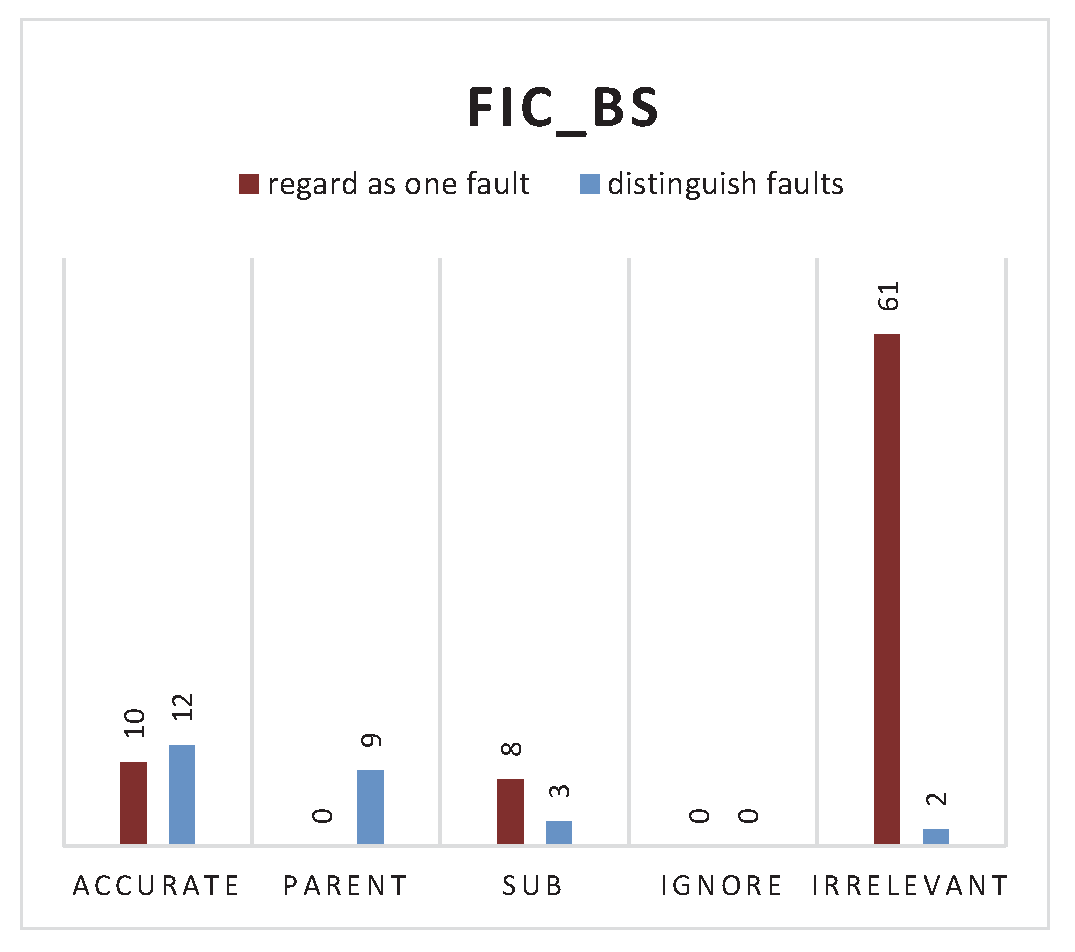
\includegraphics[width=2.21in]{FIC_BS_normal.eps}
}
\subfigure[]{
  %  \rule{4cm}{3cm}
    \label{fig:subfig2}
    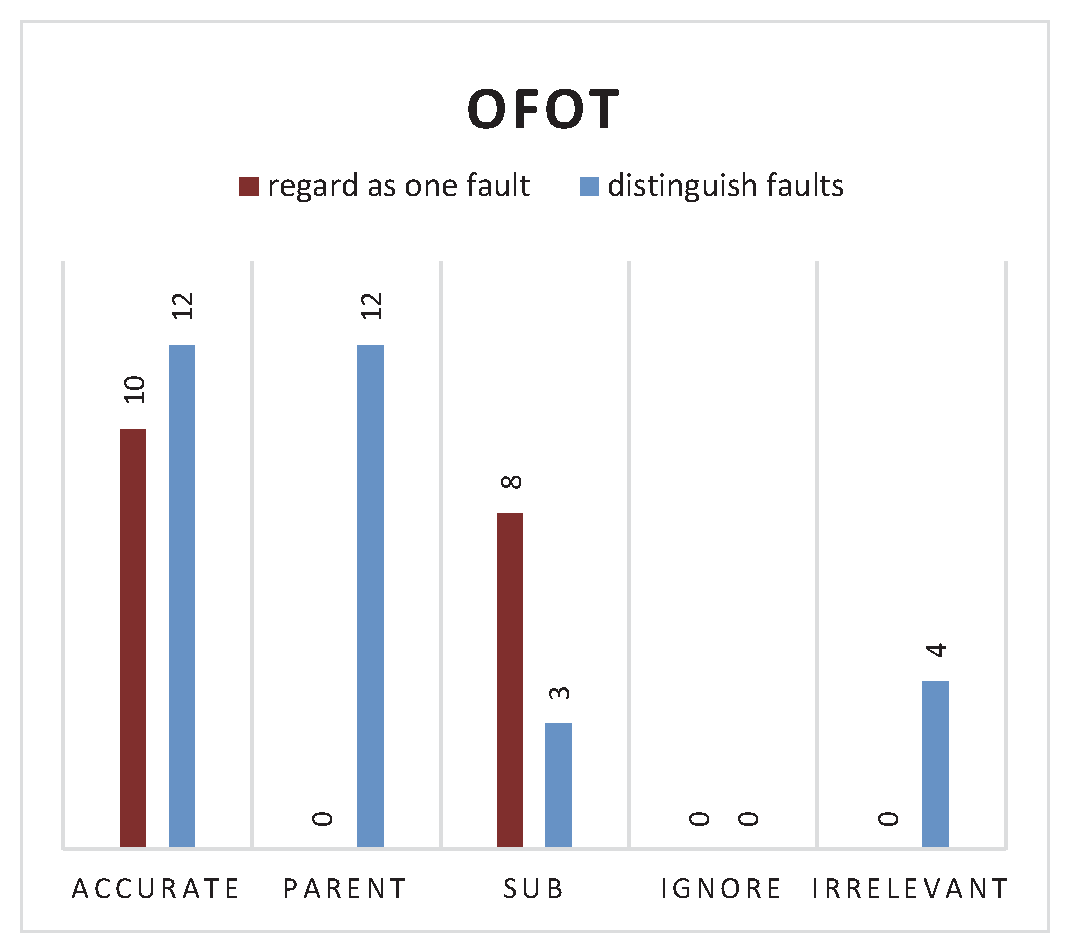
\includegraphics[width=2.21in]{OFOT_normal.eps}
}
\subfigure[]{
  %  \rule{4cm}{3cm}
    \label{fig:subfig3}
    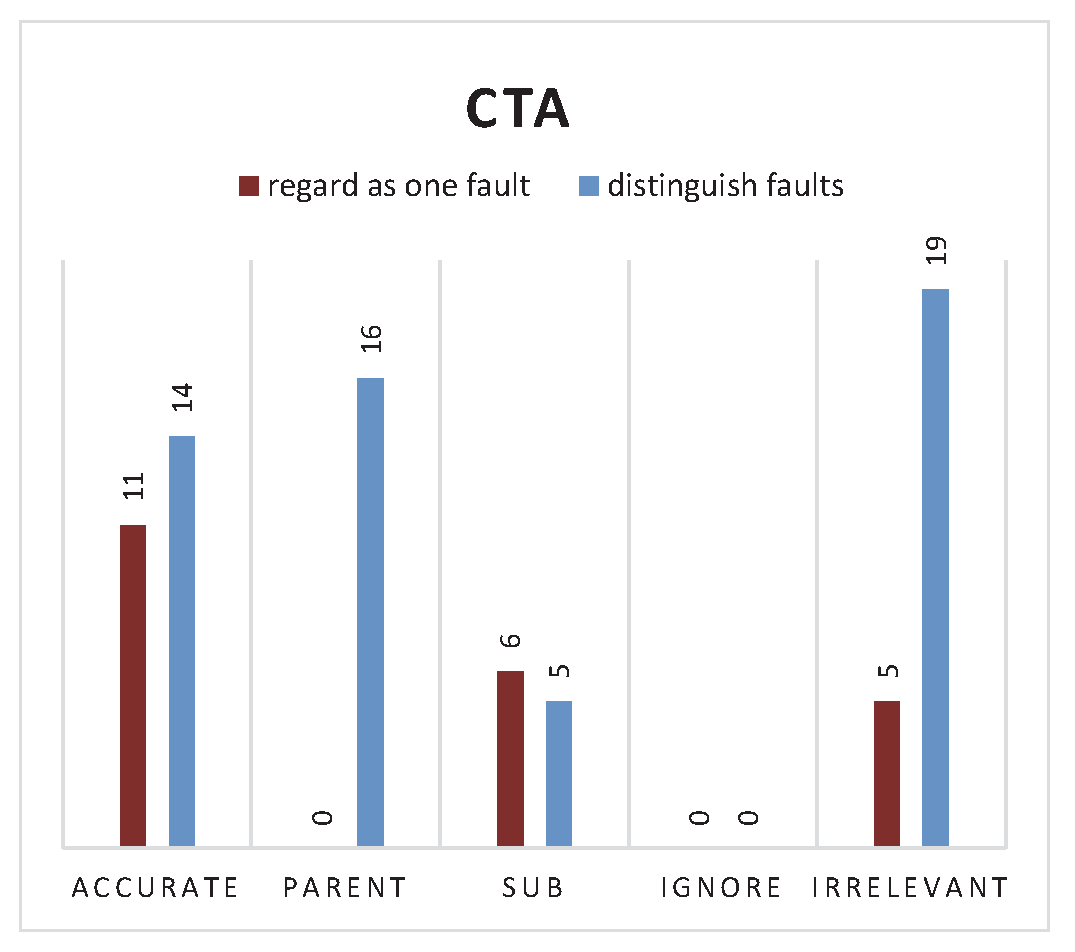
\includegraphics[width=2.21in]{CTA_normal.eps}
}
\caption[]{Results of two strategies for traditional approaches: FIC\_BS, OFOT and CTA}
\label{fig:normalexperiment}
\end{figure*}

We first observed that, traditional approaches do suffer from the masking effect to some extent. Specifically, in the Figure \ref{fig:subfig1}, FIC\_BS approach only correctly identified 12 and 10 accurate combinations for the two traditional strategies respectively, while wrongly identified 14 and 69 combinations, among which \emph{parent number}, \emph{sub number}, \emph{irrelevant number} are 9,3,2 and 0,8,61 respectively. Similar results can be observed in Figure \ref{fig:subfig2} and \ref{fig:subfig3} for approach OFOT and CTA .

Another interesting observations is that for the \emph{regard as one fault} and \emph{distinguish faults} strategy, the former get more \emph{sub combinations} than latter, while \emph{distinguish faults} strategy get more \emph{parent combinations} than \emph{regard as one} strategy. This result accorded with our formal analysis in section 3.2. With respect to the metrics \emph{irrelevant combinations}, however, we didn't get as expected as the formal analysis. In fact, both the case that \emph{regard as one fault} has more \emph{irrelevant combinations} ( see Figure \ref{fig:subfig1}) and the case that \emph{distinguish faults} obtained more \emph{irrelevant combinations} (see Figure \ref{fig:subfig2} and \ref{fig:subfig3}) exist. With checking the executing process and the combinations they got, we believed one possible main reason for this result is that the algorithm encountered the problem of importing newly faults which bias their identifying process.

%\emph{regard as one fault} would get more \emph{} except the following case,  An exception is for the FIC\_BS, which we think when consider the regard as one fault faults strategy, it increase the possibility that import newly bugs so that bais the result. it always that . fahter and parent. which are accordant with the analysis in the formal model.

We further observed that, for different algorithms, the extent to what they suffered from masking effects varied. For instance, for FIC\_BS approach, under the masking effects, they  identified the 61 and 2 irrelevant combinations for two strategies, while for OFOT and CTA, this value is 0 and 4, 5 and 19 respectively. There are two factors caused this difference: the chosen test cases and the analysis method. For FIC\_BS and OFOT, the test cases they chosen for isolating failure-inducing combinations is different, which consequently changed the masking effects they may encountered. For OFOT an CTA, while the test cases they chose are the same, the difference lies at the way they characterizing the failure-inducing combinations in the test cases: OFOT directly identify the parameter according to the passed test cases while CTA used classified tree analysis.

%
%From this figure, we can easily find that Traditional MFS identifying approaches do suffer from the multiple faults and their masking effect. For example, for the Grep, version 3.14, all these three algorithm will lost some information. Additionally, the extent to which the impact has affected vary from algorithms. We can find that for HSQLDB with version 3.14, the similarity of CTA was just at 4 while FIC is 3. We list these points in figure 3. From this figure, we can learn that.

Therefore, the answer we got for \textbf{Q2} is: traditional algorithms do suffer from the multiple faults and their masking effect, although the extent varies in different algorithms.

\subsection{Performance of our approach}
The third empirical study aims to observe the performance of our approach and compare it with the result got by the traditional approaches. Our approach augments the three traditional FCI approaches with replacing test cases strategy described in Section 4.
%, and then we applied these augmented approaches to identify the failure-inducing combinations in the prepared subjects.

\subsubsection{Study setup}
The setup of this case study is almost the same as the second case study. The difference is that the algorithms we choose are three augmented ones.

%Additionally, comparisons between the augmented approaches and three traditional ones will be quantified.

\subsubsection{Result and discussion}
Figure \ref{fig:subfigureExample2} presents the result of the last case study. The organization of this figure is similar to the second study. The bar in each column depicts the results of the augmented approaches, which is labelled as ``replacing strategy". We marked two additional points in each column which represent the result of \emph{regard as one fault} and \emph{distinguish faults} strategy to get a comparison with the augmented approaches.

% We just added some information in the parentheses attached the value in each cell. This information display the  discrepancy between traditional ones. Notation '+' means promotions against traditional ones, while '-' indicates decrease. The value in parentheses has been normalized.

\begin{figure*}[ht]
\centering
\subfigure[]{
  %  \rule{4cm}{3cm}
    \label{fig:subfig4}
    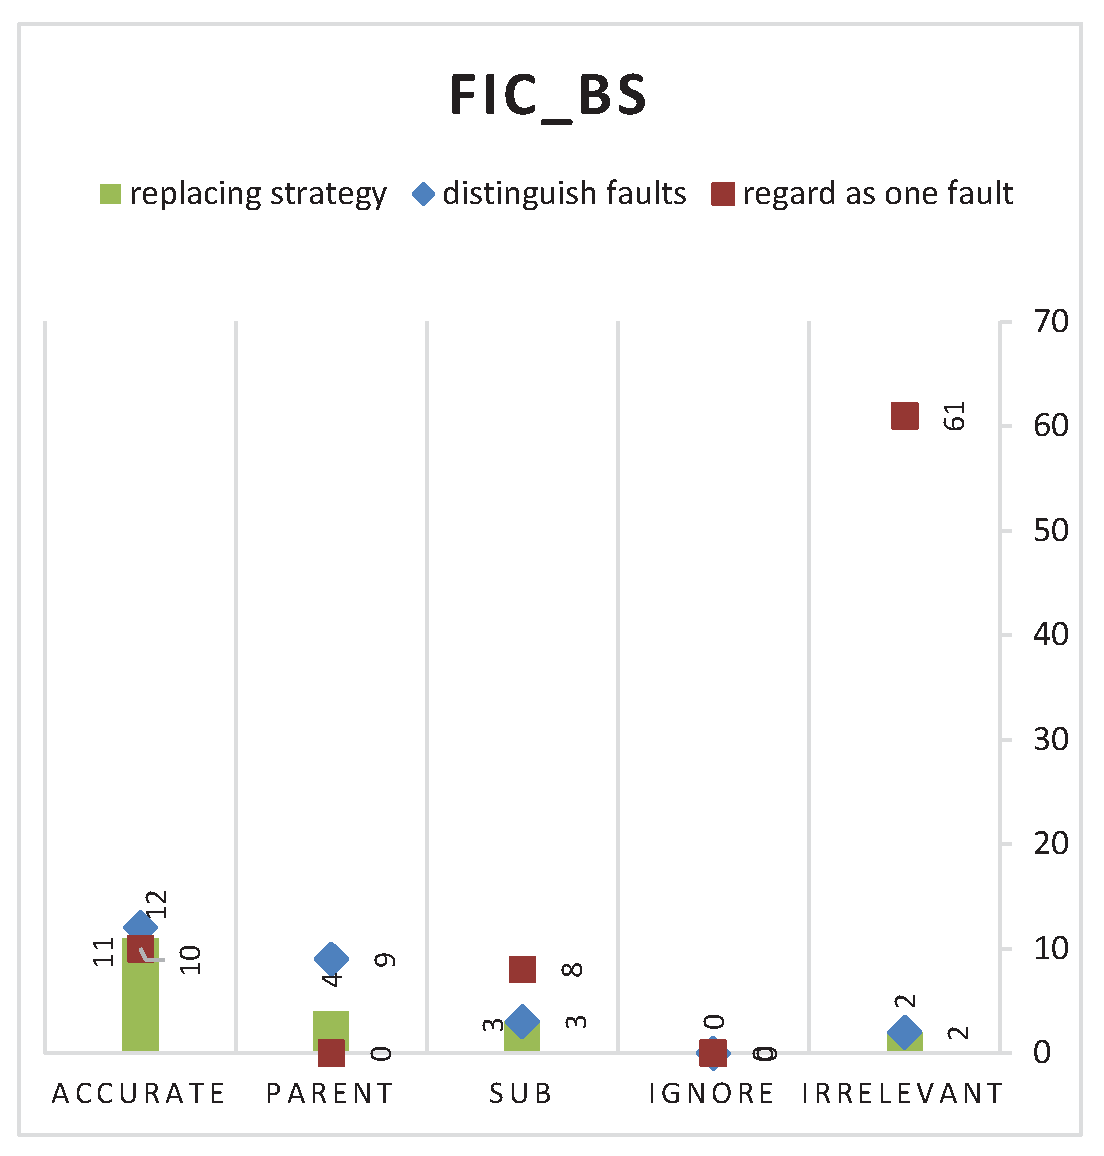
\includegraphics[width=2.21in]{FIC_BS_our.eps}
}
\subfigure[]{
  %  \rule{4cm}{3cm}
    \label{fig:subfig5}
    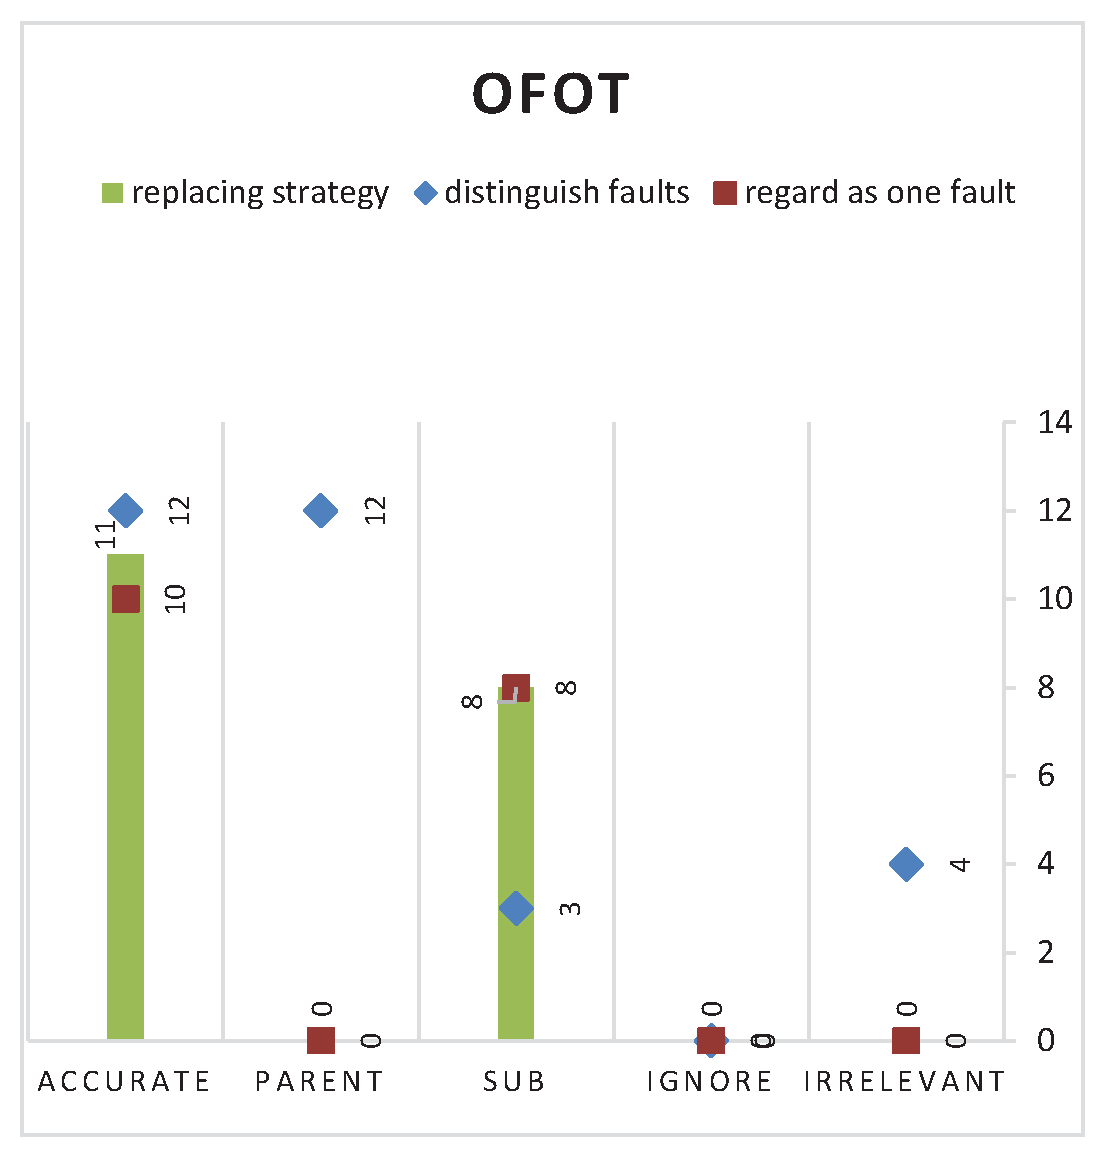
\includegraphics[width=2.21in]{OFOT_our.eps}
}
\subfigure[]{
  %  \rule{4cm}{3cm}
    \label{fig:subfig6}
    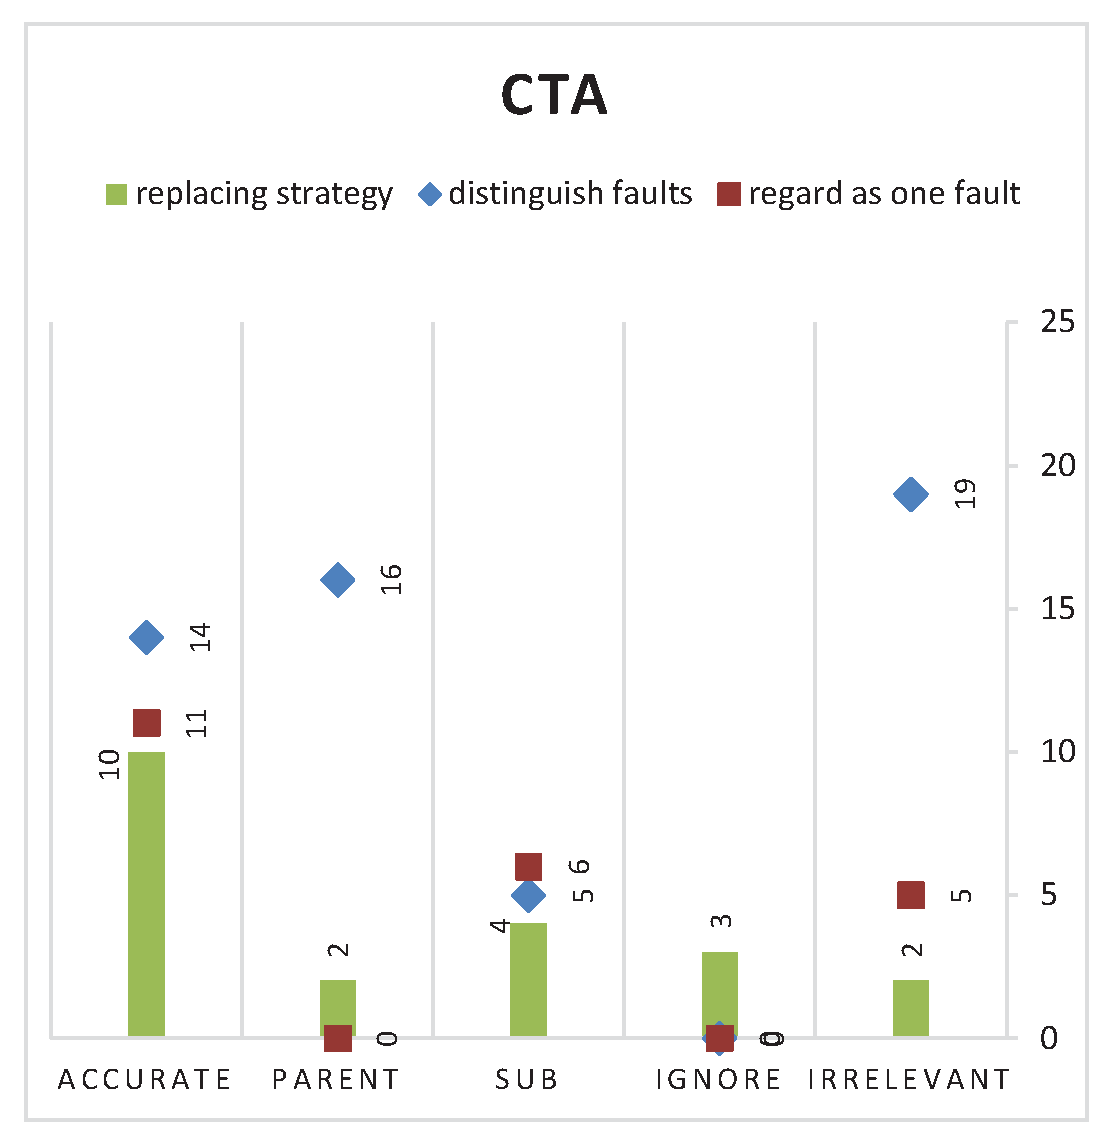
\includegraphics[width=2.21in]{CTA_our.eps}
}
\caption[Optional caption for list of figures]{Three approaches augmented with the replacing strategy}
\label{fig:subfigureExample2}
\end{figure*}


Comparing our approach with two traditional strategies in Figure \ref{fig:subfigureExample2}, we observed that there is significant improvement for augmented approaches in reducing the wrongly identified combinations. For instance, CTA approach in Figure \ref{fig:subfig6} only got 2 irrelevant combinations with replacing strategy, while the traditional two strategy got 5 and 19 irrelevant combinations respectively. And for FIC\_BS in Figure \ref{fig:subfig4} this comparison is 2 for replacing strategy, and 2 , 61 for two traditional strategies.

Besides, the augmented approaches also get a good performance at limiting the number of sub combinations and parent combination. In effect, compared with \emph{distinguish faults} which is good at limiting sub combinations while producing more parent combinations and \emph{regard as one fault} which is the other way around, the augmented ones get a more balanced result. Specifically, for instance, in Figure \ref{fig:subfig4} for approach FIC\_BS, \emph{distinguish faults} strategy obtained 9 parent combinations while got 3 sub combinations. And for \emph{regard as one fault} strategy, it got none parent combination but attained 8 sub combinations. For the replacing strategy, it only identified 4 parent combinations, which smaller than \emph{distinguish faults} strategy, and obtained 3 sub combinations which is smaller than \emph{regard as one fault} strategy and equal to \emph{distinguish faults} strategy.

Apart from these improvement, there is some slight decline for the augmented approaches in some specific situation. For example, we noted that for replacing strategy, it nearly got 2 less accurate combinations on average than traditional strategies, and ignored 1 more failure-inducing combinations on average than traditional ones.
% Further more it also that number of correctly identified combinations with replacing strategy slightly declines than traditional ones(about 2 less in average).

%As a compensation, however, We noted that the augment approaches got slightly . But promotions against traditional ones. In fact, there are 10 out of 14 cases that augment ones outperform traditional ones at the metric of "similarity", and 9 out of 14 cases that augment ones are better than traditional ones at the metric of "num diff". Additional, this promotion is distinct. As we can see, the best promotion for similarity is 0.9 and the best promotion for num diff is 0.7. Furthermore, the average performance promotion for similarity reached '+ 0.6' and this value reached '+ 0.5' for the num diff metric.

In summary, the answer for \textbf{Q3} is: our approach do make the FCI approaches, to some extent, get better better performance at identifying failure-inducing combinations when facing masking effect between multiple faults.

\subsection{Voting System}
The last empirical study aims to observe the performance of our approach and compare it with the result got by the traditional approaches. Our approach augments the three traditional FCI approaches with replacing test cases strategy described in Section 4.
%, and then we applied these augmented approaches to identify the failure-inducing combinations in the prepared subjects.

\subsubsection{Study setup}
The setup of this case study is almost the same as the second case study. The difference is that the algorithms we choose are three augmented ones.

%Additionally, comparisons between the augmented approaches and three traditional ones will be quantified.

\subsubsection{Result and discussion}



\subsection{Threats to validity}
There are several threats to validity for these empirical studies. First, we have only surveyed five open-source software, four of which are medium-sized and one is large-sized. This may impact the generality of our observations. Although we believe it is quite possible a common phenomenon in most software that contain multiple faults which can mask each other, we need to investigate more software to support our conjecture.

The second threat comes from the input model we built. As we focused on the options related to the perfect combinations and only augmented it with some noise options, there is a chance we will get different result if we choose other noise options. More different options needed to be opted to see whether our result is common or just appeared in some particular input model.

The third threats is that we just observed three failure-inducing combinations identifying algorithms, further works needed to examine more algorithms in this filed to get a more general result.

\section{related works}

Shi and Nie presented a further testing strategy for fault revealing and failure diagnosis\cite{shi2005software}, which first tests SUT with a covering array, then reduces the value schemas contained in the failed test case by eliminating those appearing in the passed test cases. If the failure-causing schema is found in the reduced schema set, failure diagnosis is completed with the identification of the specific input values which caused the failure;otherwise, a further test suite based on SOFOT is developed for each failed test cases,testing is repeated, and the schema set is then further reduced, until no more failure is found or the fault has been located . Based on this work, Wang proposed an AIFL approach which extended the SOFOT process by mutating the changing strength in each iteration of characterizing failure-inducing combinations\cite{wang2010adaptive}.

Nie et al. introduced the notion of Minimal Failure-causing Schema(MFS) and proposed the OFOT approach which extended from SOFOT that can isolate the MFS in SUT\cite{nie2011minimal}. The approach mutates one value with different values for that parameter, hence generating a group of additional test cases each time to be executed. Compared with SOFOT, this approach  strengthen the validation of the factor under analysis and also can detect the newly imported faulty combinations.

Delta debugging \cite{zeller2002simplifying} proposed by Zeller is an adaptive divide-and-conquer approach to locate interaction fault. It is very efficient and has been applied to real software environment. Zhang et al. also proposed a similar approach that can identify the failure-inducing combinations that has no overlapped part efficiently \cite{zhang2011characterizing}. Later Li improved the delta-debugging based failure-inducing combination by exploiting the useful information in the executed covering array\cite{li2012improved}.

Colbourn and McClary proposed a non-adaptive method \cite{colbourn2008locating}. Their approach extends the covering array to the locating array to detect and locate interaction faults. C. Martinez proposed two adaptive algorithms. The first one needs safe value as their assumption and the second one remove the assumption when the number of values of each parameter is equal to 2\cite{martinez2008algorithms,martinez2009locating}. Their algorithms focus on identifying the faulty tuples that have no more than 2 parameters.

Ghandehari et al. defined the suspiciousness of tuple and suspiciousness of the environment of a tuple\cite{ghandehari2012identifying}. Based on this, they rank the possible tuples and generate the test configurations. They further utilized the test cases generated from the inducing combination to locate the faults inside the source code\cite{ghandehari2013fault}.

Yilmaz proposed a machine learning method to identify inducing combinations from a combinatorial testing set \cite{yilmaz2006covering}. They construct a classified tree to analyze the covering arrays and detect potential faulty combinations. Beside this, Fouch{\'e} \cite{fouche2009incremental} and Shakya \cite{shakya2012isolating} made some improvements in identifying failure-inducing combinations based on Yilmaz's work.

Our previous work \cite{niu2013identifying} have proposed an approach that utilize the tuple relationship tree to isolate the failure-inducing combinations in a failing test case. One novelty of this approach is that it can identify the overlapped faulty combinations. This work also alleviates the problem of introducing newly failure-inducing combinations in additional test cases.

In addition to the works that aims at identifying the failure-inducing combinations in test cases, there are some studies focus on working around the masking effects:

With having known masking effects in prior, Cohen \cite{cohen2007exploiting,cohen2007interaction,cohen2008constructing} studied the impacts that the masking effects render some generated test cases invalid in CT, and they proposed the approach that integrate the incremental SAT solver with covering array generating algorithms to avoid these masking effects in test cases generating process. Further study was conducted \cite{petke2013efficiency}to show the fact that with considering constrains, the higher-strength covering arrays with early fault detection is practical. Besides, additional constraints impacts in CT were studied in works like \cite{garvin2011evaluating,bryce2006prioritized,calvagna2008logic,grindal2006handling,yilmaz2013test}. %These approaches use some rules or to avoid these invalidated test cases to improve the efficiency when examine the test cases.

Chen et al. addressed the issues of shielding parameters in combinatorial testing and proposed the Mixed Covering Array with Shielding Parameters (MCAS) to solve the problem caused by shielding parameters\cite{chen2010combinatorial}. The shielding parameters can disable some parameter values to expose additional interaction errors, which can be regarded as a special case of masking effects.

Dumlu and Yilmaz proposed a feedback-driven approach to work around the masking effects\cite{dumlu2011feedback}. In specific, it first use CTA classify the possible failure-inducing combinations and then eliminate them and generate new test cases to detect possible masked interaction in the next iteration. They further extended their work \cite{yilmaz2013reducing}, in which they proposed a multiple-class CTA approach to distinguish faults in SUT. In addition, they empirically studied the impacts on both ternary-class and multiple-class CTA approaches.

Our work differs from these ones mainly in the fact that we formally studied the masking effects on FCI approaches and further proposed a divide-and-conquer strategy to alleviate this impact.

\section{Conclusions}
Masking effects of multiple faults in SUT can bias the result of traditional failure-inducing combinations identifying approaches. In this paper, we formally analysed the impact of masking effects on FCI approaches and showed that both two traditional strategies are inefficient in handling such impact. We further presented a divide and conquer strategy for FCI approaches to alleviate this impact.

%This strategy separately handle each fault in SUT, and for a particular fault, it will discard these test cases that trigger faults different from the one under analysis and only keep those that either pass or trigger the expected fault. Additional test cases for compensation will be generated after discarding unsatisfied test cases.

In the empirical studies, we extended three FCI approaches with our strategy. The comparison between this three traditional approaches and their improved variations was conducted on several open-source software. The results indicated that our strategy do assist traditional FCI approaches in getting a better performance when facing masking effects in SUT.

As a future work, we need to do more empirical studies to make our conclusion more general. Our current experimental subjects are several middle-sized software, we would like to extend our approach into more complicated and large-scaled testing scenarios. Another promising work in the future is to combine white-box testing technique to make the FCI approaches get more accurate results when handling masking effects. We believe that figuring out the fault levels of different bugs through white-box testing technique is helpful to reduce misjudgement in the failure-inducing combinations identifying process. At last, as the extent to what the FCI suffers from masking effects varies in different algorithms, the combination of different FCI approaches is desired in the future to further improve the performance for identifying failure-inducing combinations for multiple faults.



% Start of "Sample References" section

\section{Typical references in new ACM Reference Format}
%A paginated journal article \cite{Abril07}, an enumerated
%journal article \cite{Cohen07}, a reference to an entire issue \cite{JCohen96},
%a monograph (whole book) \cite{Kosiur01}, a monograph/whole book in a series (see 2a in spec. document)
%\cite{Harel79}, a divisible-book such as an anthology or compilation \cite{Editor00}
%followed by the same example, however we only output the series if the volume number is given
%\cite{Editor00a} (so Editor00a's series should NOT be present since it has no vol. no.),
%a chapter in a divisible book \cite{Spector90}, a chapter in a divisible book
%in a series \cite{Douglass98}, a multi-volume work as book \cite{Knuth97},
%an article in a proceedings (of a conference, symposium, workshop for example)
%(paginated proceedings article) \cite{Andler79}, a proceedings article
%with all possible elements \cite{Smith10}, an example of an enumerated
%proceedings article \cite{VanGundy07},
%an informally published work \cite{Harel78}, a doctoral dissertation \cite{Clarkson85},
%a master's thesis: \cite{anisi03}, an online document / world wide web resource \cite{Thornburg01}, \cite{Ablamowicz07},
%\cite{Poker06}, a video game (Case 1) \cite{Obama08} and (Case 2) \cite{Novak03}
%and \cite{Lee05} and (Case 3) a patent \cite{JoeScientist001},
%work accepted for publication \cite{rous08}, 'YYYYb'-test for prolific author
%\cite{SaeediMEJ10} and \cite{SaeediJETC10}. Other cites might contain
%'duplicate' DOI and URLs (some SIAM articles) \cite{Kirschmer:2010:AEI:1958016.1958018}.
%Boris / Barbara Beeton: multi-volume works as books
%\cite{MR781536} and \cite{MR781537}.

% Appendix
\appendix
\section*{APPENDIX}
\setcounter{section}{1}


\appendixhead{ZHOU}

% Acknowledgments
\begin{acks}
The authors would like to thank Dr. Maura Turolla of Telecom
Italia for providing specifications about the application scenario.
\end{acks}

% Bibliography
\bibliographystyle{ACM-Reference-Format-Journals}
\bibliography{acmsmall-sample-bibfile}
                             % Sample .bib file with references that match those in
                             % the 'Specifications Document (V1.5)' as well containing
                             % 'legacy' bibs and bibs with 'alternate codings'.
                             % Gerry Murray - March 2012

% History dates
\received{February 2007}{March 2009}{June 2009}

% Electronic Appendix
\elecappendix

\medskip

\section{This is an example of Appendix section head}


\section{Appendix section head}

The primary consumer of energy in WSNs is idle listening. The key to
reduce idle listening is executing low duty-cycle on nodes. Two
primary approaches are considered in controlling duty-cycles in the
MAC layer.

\end{document}
% End of v2-acmsmall-sample.tex (March 2012) - Gerry Murray, ACM


